%! Mode:: "TeX:UTF-8"
%! TEX program = xelatex
\PassOptionsToPackage{quiet}{xeCJK}
\documentclass[withoutpreface,bwprint]{cumcmthesis}
\usepackage{etoolbox}
%\BeforeBeginEnvironment{tabular}{\zihao{-5}}
\usepackage[framemethod=TikZ]{mdframed}  % 框架宏包
\usepackage{url}  % 网页链接宏包
\usepackage{setspace}
\usepackage{graphicx}
%%%%%%%%%%%%%%%%%%%%%%%%%%%%%%%%%%%%%%%%%%%%%%%%%%%%%%%%
%下面是美赛搬过来的usepackage
\usepackage{pgfplots}
\pgfplotsset{compat=1.18}
%\usepackage{palatino}  % 帕拉提诺体字体宏包
%\usepackage{times}  % 正文使用Times New Roman风格字体
%\usepackage{newtxmath}
\usepackage{lipsum}  % 导入生成段落的宏包
\usepackage{indentfirst}
\usepackage{booktabs} % For professional-looking tables
\usepackage{xcolor}   % For cell coloring
\usepackage{colortbl} % Required for \rowcolor
\definecolor{LightGreen}{rgb}{0.9, 0.95, 0.9}
\definecolor{LightBlue}{RGB}{229, 238, 255}
\definecolor{LightPink}{RGB}{255, 229, 237}
\usepackage{fancyhdr}
\usepackage{enumitem} % 用于自定义列表格式
\usepackage{setspace}
\usepackage{booktabs}  % 三线表加粗
\usepackage{float}
\usepackage{eso-pic}  % 用于在页面添加背景
\usepackage{graphicx} % 图片支持
\usepackage{tikz}     % 用于绘制半透明覆盖层
\usepackage{subcaption}
\usepackage{caption}
\setlist[itemize]{listparindent=2em}
\setlist[enumerate]{listparindent=2em}
\setlength\parindent{2em}
\usepackage[titles]{tocloft}
\usepackage{tabularx}
\usepackage[titles]{tocloft}
\setlength{\cftbeforesecskip}{8pt}   % 节前间距
\setlength{\cftbeforesubsecskip}{4pt} % 小节前间距

\makeatletter
\renewcommand{\@seccntformat}[1]{\csname the#1\endcsname\hspace{1em}}
\makeatother%这四行是调subsub的空格

% 设置中文字体加粗使用黑体
\setCJKfamilyfont{bfsong}[AutoFakeBold=2]{SimHei}
\renewcommand{\bfseries}{\CJKfamily{bfsong}}


\urlstyle{rm}
\setlength{\headheight}{13.6pt}
\lstset{
    basicstyle=\footnotesize\ttfamily, % 字体大小和类型
    numbers=left,               % 在左侧显示行号
    numberstyle=\tiny,          % 设置行号字体
    numbersep=5pt,              % 行号与代码间距
    showspaces=false,           % 不显示空格
    showstringspaces=false,     % 字符串中不显示空格
    showtabs=false,             % 不显示制表符
    tabsize=2,                  % 制表符大小
    breaklines=true,            % 自动换行
    breakatwhitespace=false,    % 只在空格处换行
    title=\lstname,             % 显示文件名
    escapeinside={\%*}{*)},     % LaTeX代码嵌入
    xleftmargin=10pt,           % 左边距
    xrightmargin=10pt,          % 右边距
    aboveskip=5pt,              % 上方间距
    belowskip=5pt,              % 下方间距
    lineskip=-1pt               % 减小行距（负值可以压缩行距）
}
\newcolumntype{C}{>{\centering\arraybackslash}X}
\newcolumntype{R}{>{\raggedleft\arraybackslash}X}
\newcolumntype{L}{>{\raggedright\arraybackslash}X}
\renewcommand{\abstractname}{摘\kern1em要}
\title{基于时间序列预测与线性规划的微网购电优化策略}  % 论文标题
\tihao{}  % 题号
\baominghao{}  % 报名号
\schoolname{}  % 学校
\membera{}  % 队员a
\memberb{}  % 队员b
\memberc{}  % 队员c
\supervisor{}  % 指导老师
\yearinput{}
\monthinput{}
\dayinput{}

%%%%%%%%%%%%%%%%%%%%%%%%%%%%%%%%%%%%%%%%%%%%%%%%%%%%%%%%%%%%%
%% 正文
\begin{document}

\maketitle
\begin{abstract}

在现代微网负荷调控中，小区需要用电而形成整体负载，小区自身有光伏发电，但不能时刻满足小区供电，于是需要向外网购电。负载与电价会实时波动，为了供给负载并节省购电费用，储能设备与微网购电的调控成为了关键问题。依据某小区一年负载、光伏发电与电价的实时监测情况，本文主要研究回应用电、发电情况的规律、制定小区购电费用最小的微网购电方案。通过\textbf{线性规划}、\textbf{MSTL时间序列分解}等进行求解。

\textbf{针对问题一}：以全天购电费最小为目标，根据题目电力收支平衡、首末储电量相同等作为约束条件，采用\textbf{线性规划}求解。结果显示，最终策略整体体现出在电费低谷多买、电费高峰不买的特征。全天购电费为\textbf{35126.95元}。

\textbf{针对问题二}：分为预测与优化两部分。对于\textbf{负载预测}，根据早晚高峰，工作日与周末，全年缓慢升降的用电规律，用 MSTL 把负载分解为趋势、日周期、周周期与残差四部分。对于\textbf{光伏预测}，由于太阳周年运动与日内太阳高度变化，定义季节晴空强度 $B^{\mathrm{PV}}_{d,t}$；由于云层、雾霾等天气因素，定义日透射率 $\kappa_d\in[0,1]$。
由于相邻天气过程通常具有一定持续性，使用 AR($p$)对$\kappa$做日尺度滚动预测。
所有分解得到的残差仍具有显著自相关性，则用AR($p$)模型把残差进一步分解为短期自相关部分和白噪声
。对于紧急购电价格高而导致的\textbf{风险不对称}，我们对扣除光伏发电的净负荷高于预测的正向偏差提取历史加权分位数,作为应对供电低于负载时的“备用电”，并利用\textbf{报童模型}根据缺电与多电的边际代价之比动态调整分位水平，使备用量自适应地向代价更高的缺电侧倾斜。
\textbf{优化部分}框架与第一问相同，目标函数变为紧急购电费、窗口跨入次日时按正常电价计费的虚拟购电费。结果显示符合与光伏功率预测准确，全年紧急购电费仅占3.37\%。



\textbf{针对问题三}：首先通过线性插值处理预报以1h为单位与模型以10min为单位的匹配问题。随后基于问题二，把购电调整分解为向上与向下两部分：$P^{\mathrm{buy}}_{k,t}=P^{\mathrm{buy}}_{k-1,t}+U^{+}_{k,t}-U^{-}_{k,t}$，分别按 $1.5\lambda_t U^{+}_{k,t}\Delta t$ 与 $0.5\lambda_t U^{-}_{k,t}\Delta t$ 分别计入追加和违约费用。最终结果显示，经过预报，向下调整总电费占总调整电费的78.99\%。对于引入其他时刻的预报，我们构造了光伏功率的\textbf{动态非对称风险带}。由于预测偏高易触发高价的紧急购电，风险带的危险侧容许宽度更窄。随后，我们通过预测值偏离带状区域的越界量筛选出需要增加额外预报的候选时点，再把时点代入预测模型，根据最后的全年购电费是否降低等来判断是否引入候选时点。最终结果建议不添加预报时点。

\textbf{针对问题四}：由于电价也具有日周期与周周期特征，我们沿用MSTL结合AR模型，构建电价预测模型。随后通过实时更新的电价做轻量级指数加权残差修正以实现滚动更新。优化框架沿用前两问设计，只改变目标函数中的电价为预测电价，最后用实际电价计算总购电费用。对于引入预报时点，将电价与光伏两类同时纳入联合风险，将局部可提供信息价值最大的时点纳入候选时点。最终建议不添加预报时点。




\keywords{微网购电\quad 线性规划\quad MSTL时间序列分解\quad AR($p$)自回归\quad 报童模型}
\end{abstract}
%%%%%%%%%%%%%%%%%%%%%%%%%%%%%%%%%%%%%%%%%%%%%%%%%%%%%%%%%%%%% 

% \tableofcontents  % 目录
% \newpage

%%%%%%%%%%%%%%%%%%%%%%%%%%%%%%%%%%%%%%%%%%%%%%%%%%%%%%%%%%%%%  
\section{问题重述}
\subsection{问题背景}
\vspace{-5pt}
随着分布式能源的快速发展，配备储能设备的微网可通过“低充高放”有效降低整体购电费用。然而，小区负载、光伏发电和外部电价均随时间波动，且储能设备存在容量、功率与效率等物理限制。如何在满足用电需求的前提下合理安排购电与充放电策略，并应对光伏预报更新与电价波动带来的调控复杂性，是实现微网经济运行的关键。

%%%%%%%%%%%%%%%%%%%%%%%%%%%%%%%%%%%%%%%%%%%%%%%%%%%%%%%%%%%%% 
\vspace{-13pt}
\subsection{问题提出}

某微网由小区负载、光伏发电、储能设备及外部电网购电组成。题目附件提供了全年的负载与光伏实际功率、多时点的光伏功率预报、波动电价，以及储能设备的物理参数（包括最大容量、充放电功率限制、初始电量、安全运行区间及充放电效率等）。现需结合上述信息建立数学模型，分析以下问题：

\textbf{问题一}：为了在电价和小区负载每天相同、光伏发电功率预测数据已知的情形下制定微网当天的计划购电策略，需要满足以下条件，给出计划购电量与储能设备充放电方案：

\begin{enumerate}[label=\arabic*.,leftmargin=40pt]
	
	\item 保证微网提供的电能不低于小区负载
	\item 满足储能设备最大容量、最大充放电功率、安全电量区间和充放电效率等约束
	\item 使储能设备在0:00和24:00的储电量相同
	\item 以全天购电费用最小为目标
	
\end{enumerate}

\textbf{问题二}：在每天电价相同，而小区负载和光伏发电实际功率随时间变化的情形下，制定微网当天计划购电策略，需要综合考虑以下因素，从而给出指定日期的计划购电量、储能设备充放电量和紧急购电量：

\begin{enumerate}[label=\arabic*.,leftmargin=40pt]
	
	\item 微网提供的电能不可低于小区负载
	\item 若实际供电低于小区负载，需向外网紧急购电，紧急购电电价为交易时刻电价的5倍
	\item 除紧急购电费用外，其他时间段的购电费用按计划购电量计算
	
\end{enumerate}

最后使用构建的模型给出完整购电策略，并保存相应结果。

%\hangindent=72pt
\textbf{问题三}：在每天0:00、6:00、12:00和18:00可获得未来24小时整点光伏发电功率预报的条件下，微网可根据0:00预报制定当天计划购电策略，也可根据其他时刻的预报调整购电策略。调整购电策略会带来两类费用后果：若计划购电量高于调整购电量，高出部分按交易时刻电价的50\%承担违约费用；若调整购电量高于计划购电量，高出部分按交易时刻电价的1.5倍计费。需要以当天总购电费用最小为目标，给出计划购电策略与调整购电策略，并分析是否需要引入其他时刻的预报。

%\hangindent=70pt
\textbf{问题四}：针对外部电网电价实时波动的实际情况，与二三问相同，需要对每日电价进行预测，在波动电价下重新计算问题二和问题三。



%%%%%%%%%%%%%%%%%%%%%%%%%%%%%%%%%%%%%%%%%%%%%%%%%%%%%%%%%%%%% 

\section{问题分析}

\begin{figure}[h!]
	\centering
	% trim = 左边裁剪 下边裁剪 右边裁剪 上边裁剪（单位：cm）
	% clip 表示启用裁剪功能
	\vspace{0cm}
	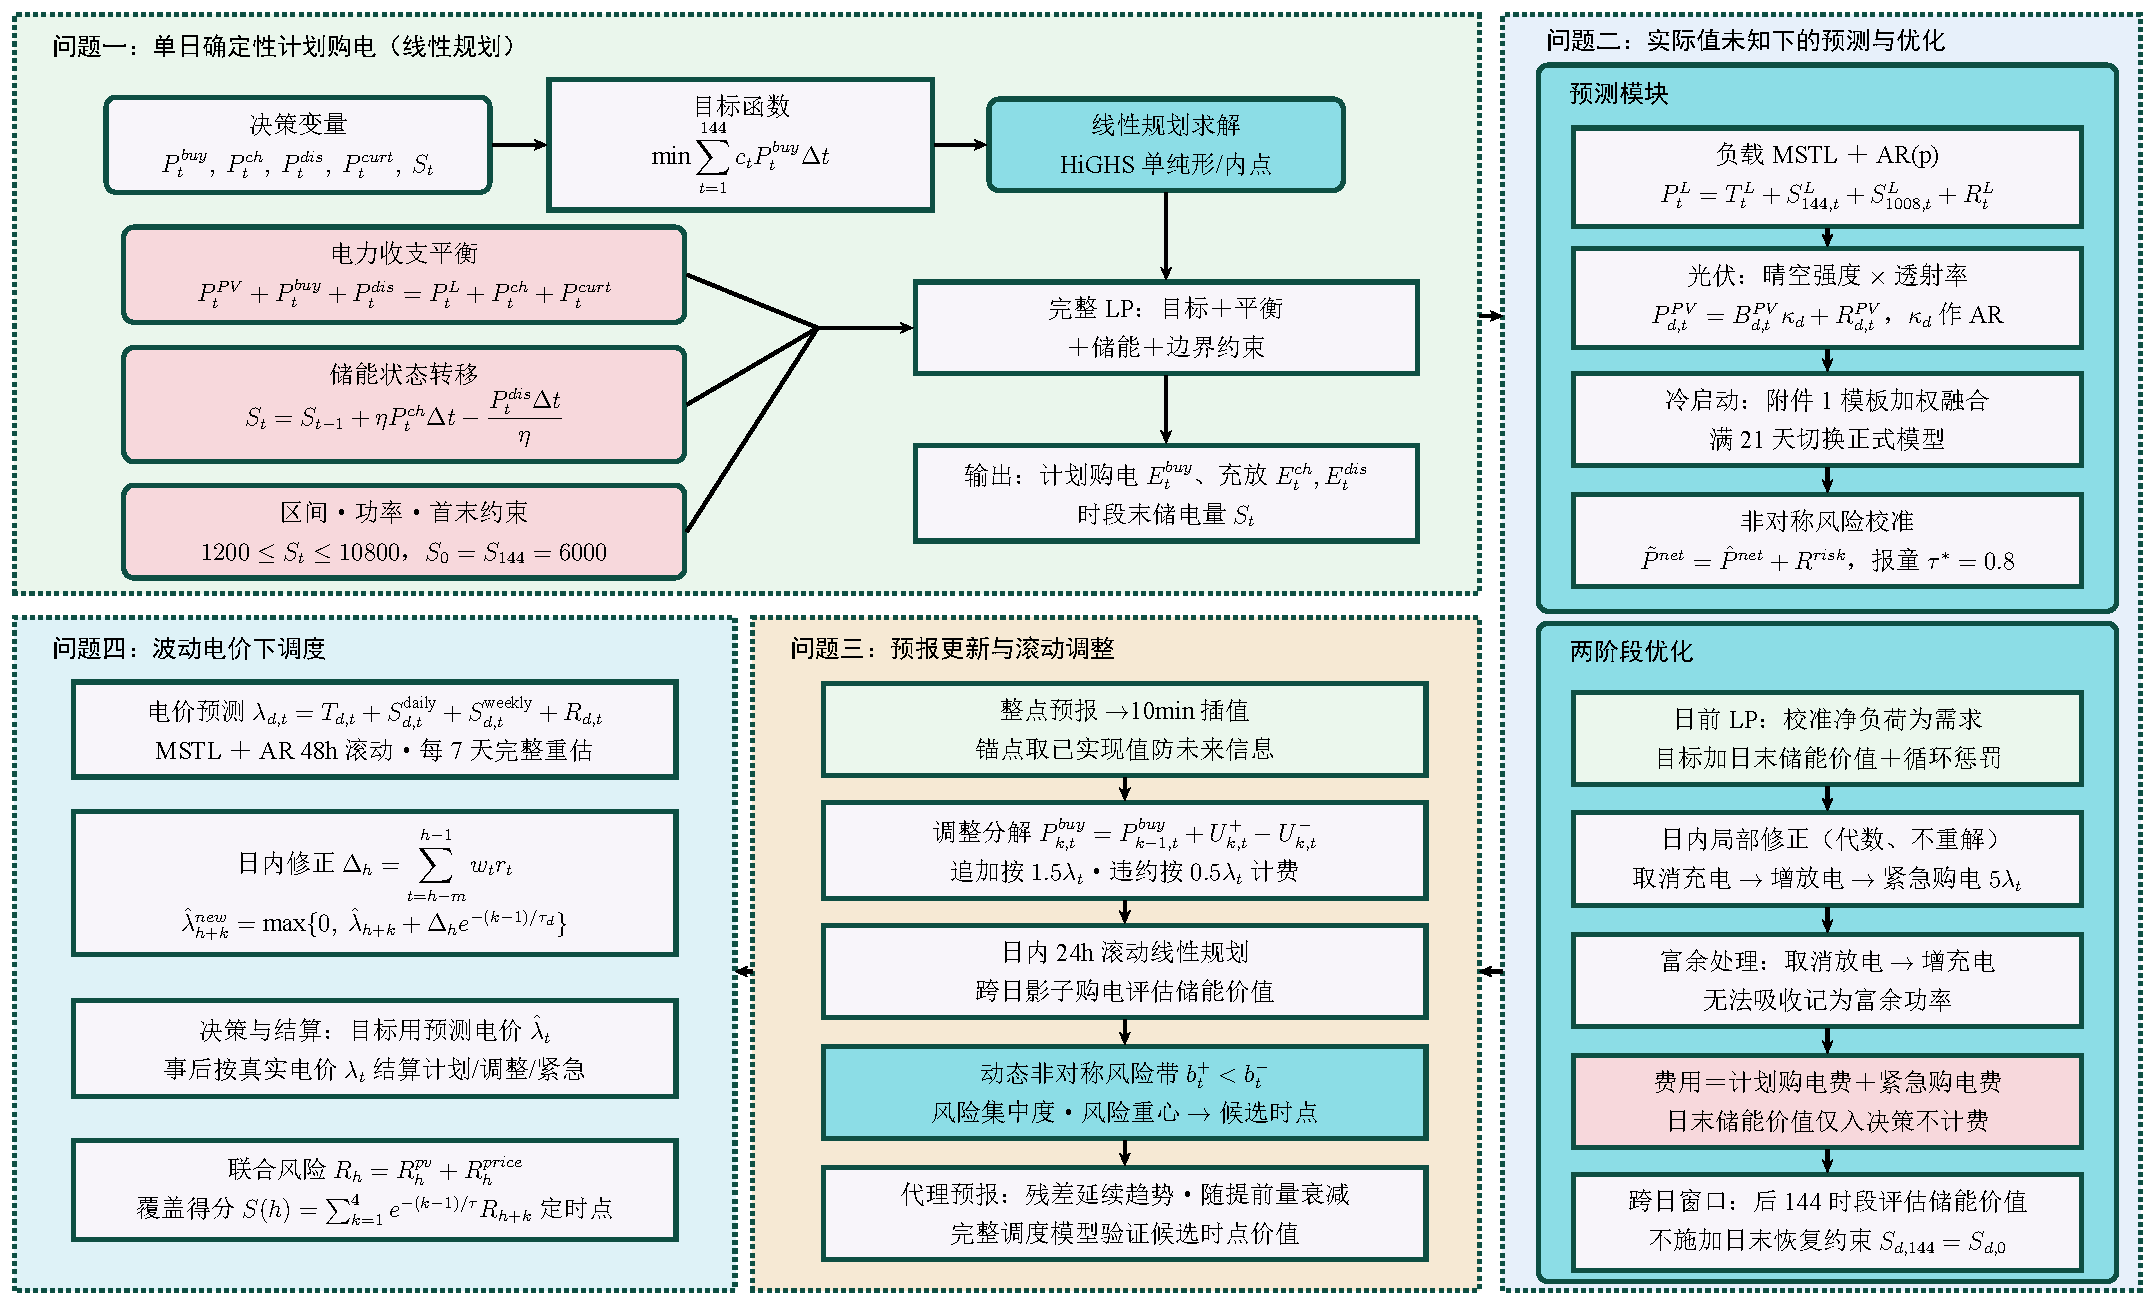
\includegraphics[
	width=1\textwidth,
	trim=0cm 0cm 0cm 0cm, 
	clip
	]{figures/26国赛流程图.pdf}
	\caption{问题求解流程图}
	\label{fig:26国赛流程图.pdf}
\end{figure}

\vspace*{-15pt}
\subsection{问题一分析}
%\begin{figure}[ht]
%\centering
%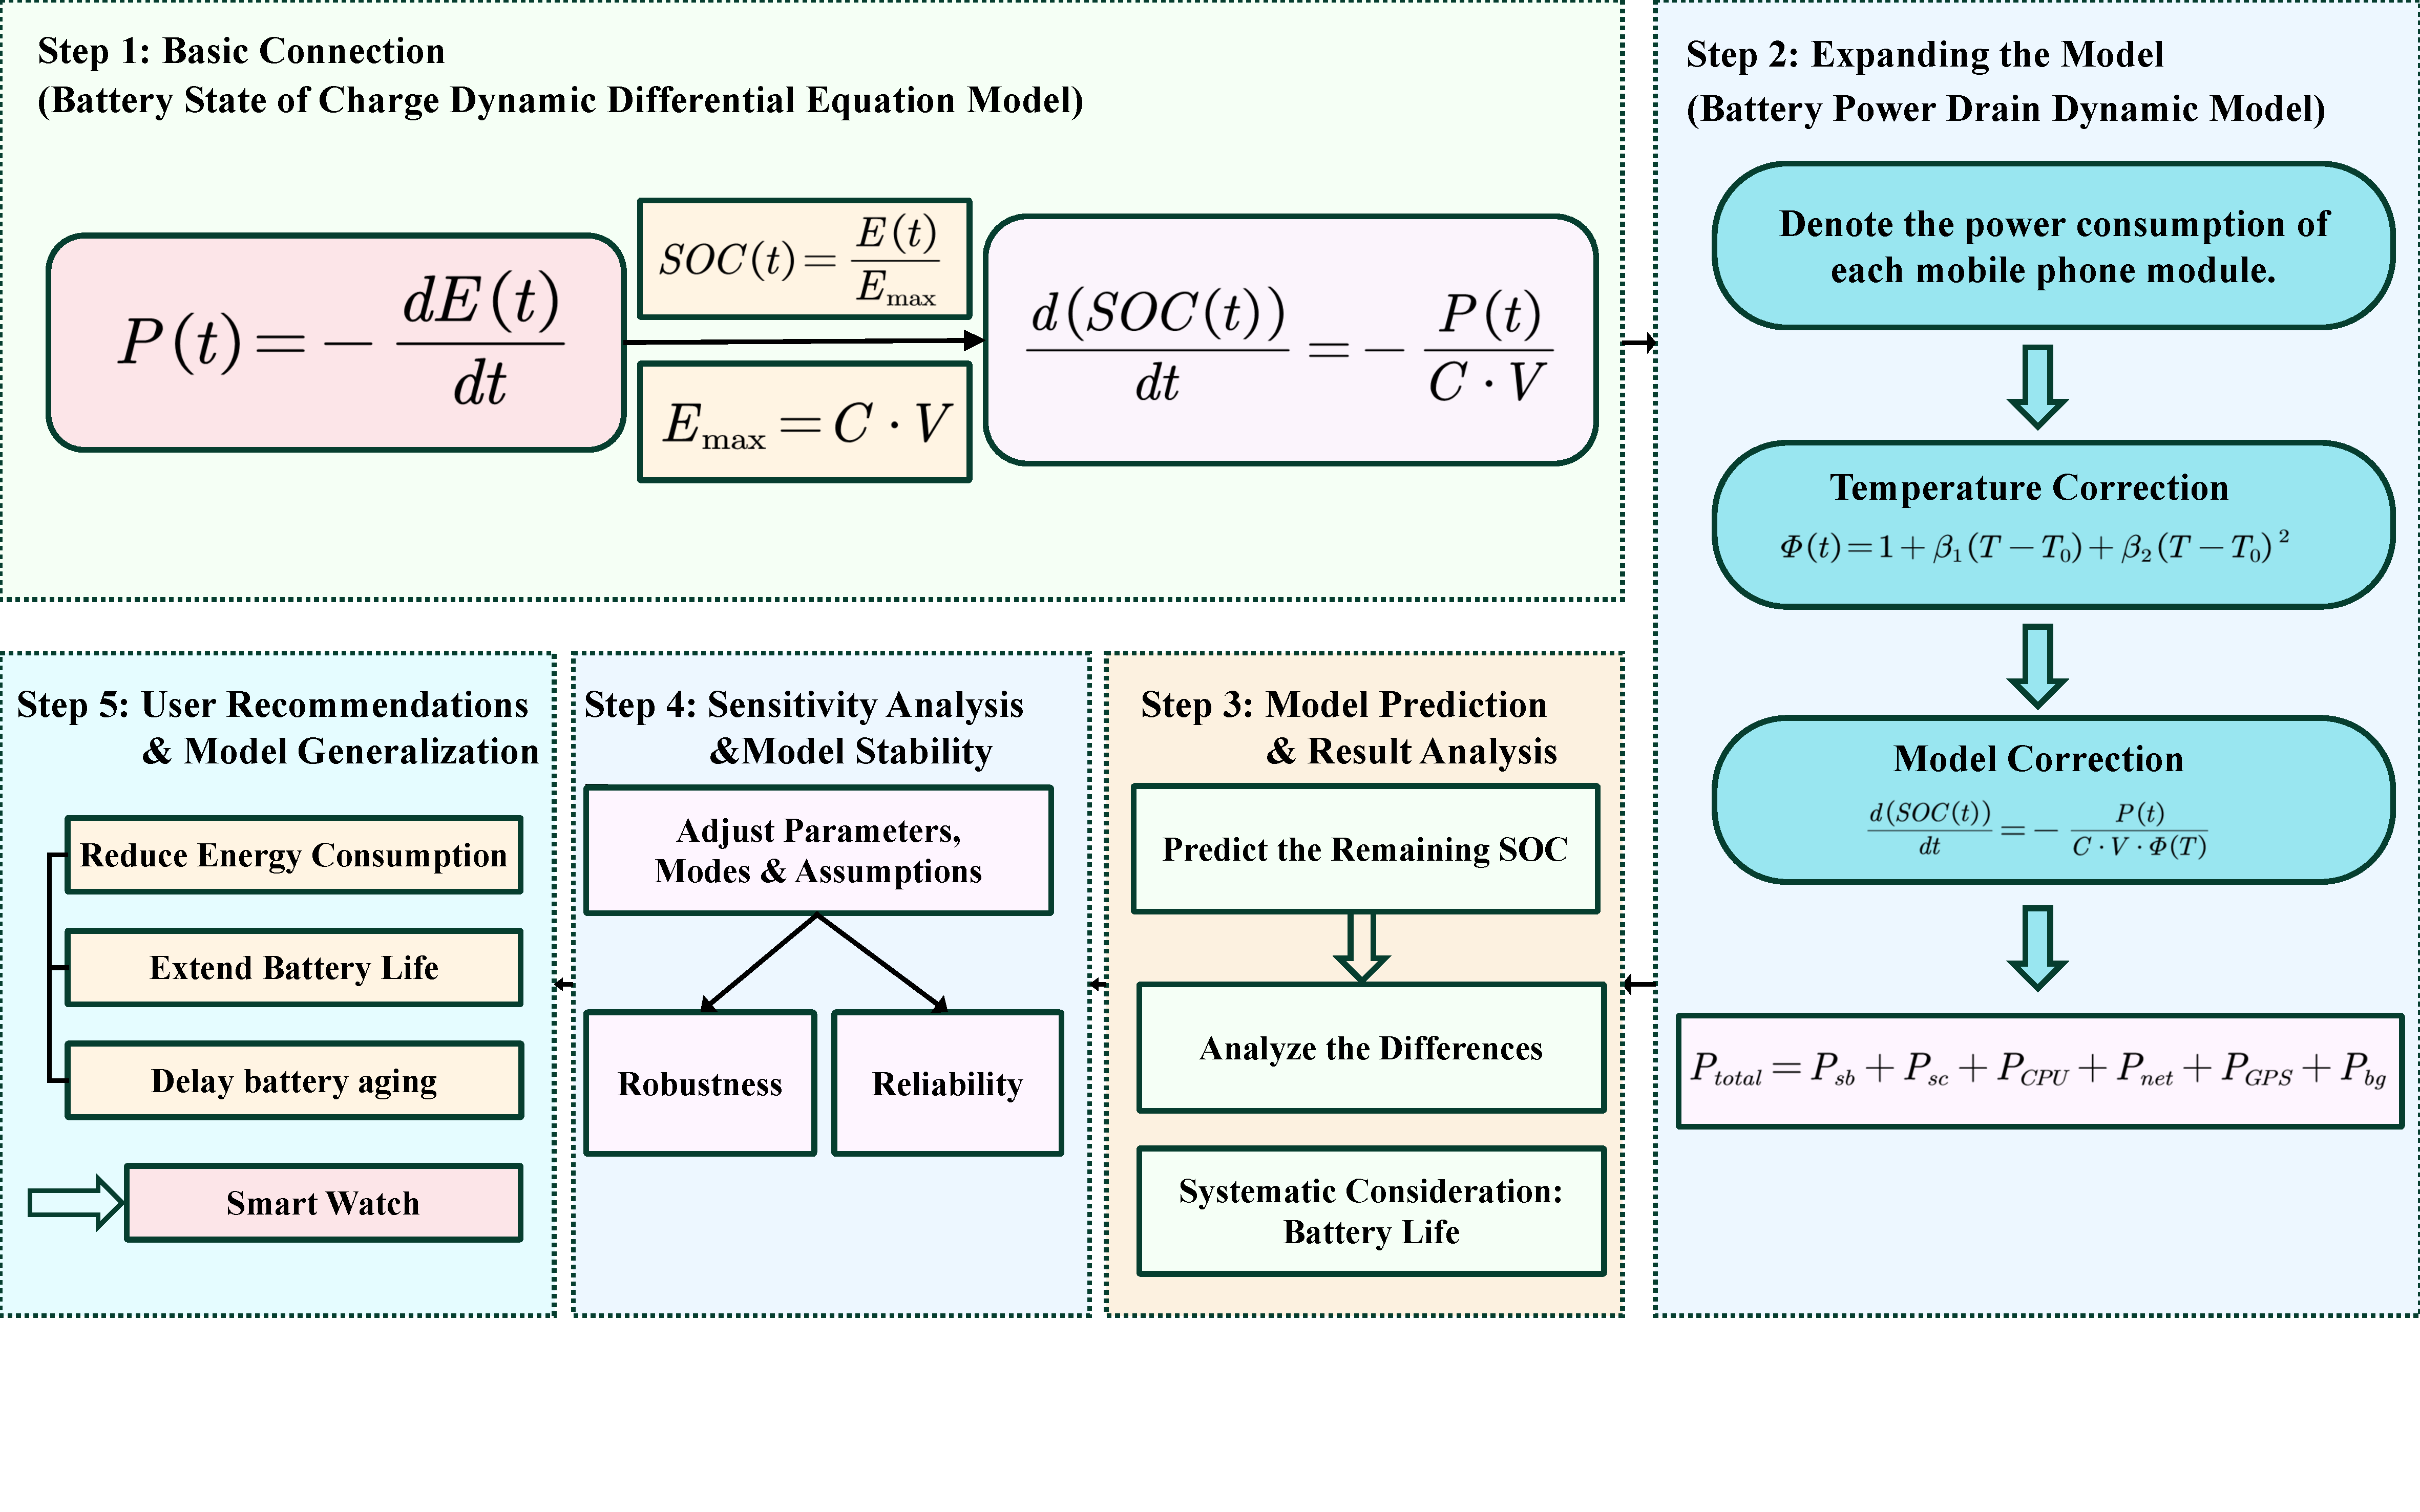
\includegraphics[width=1.05\textwidth,trim=0cm 6.5cm 0cm 0cm, 
%clip]{figures/2026美赛流程图.pdf}
%\caption{问题一分析流程图}
%\label{fig:问题一分析}
%\end{figure}




问题 1 要求在给定电价、小区负载和光伏发电预测功率的条件下，制定微网当天的计划购电与储能设备充放电方案，属于单日调度优化问题。首先，确定决策变量为一天 144 个 10 分钟时段的购电量 \(E^{\mathrm{buy}}_t\)、储能设备充放电量 \(E^{\mathrm{ch}}_t\) 与 \(E^{\mathrm{dis}}_t\)，以及各时段末储电量 \(S_t\)。接着，以全天购电费用最小为目标： \(\min \sum_{t=1}^{144} c_t E^{\mathrm{buy}}_t\)。随后建立约束条件：电力收支平衡约束、供电可靠性约束、储能设备充放电功率约束、储电量状态转移与区间约束、首末储电量约束。由于目标函数与各类约束均为线性关系，利用线性规划模型即可求解得到计划购电策略与储能设备充放电策略。



\vspace*{-20pt}
\subsection{问题二分析}	
%\begin{figure}[h!]
%	\centering
%	% trim = 左边裁剪 下边裁剪 右边裁剪 上边裁剪（单位：cm）
%	% clip 表示启用裁剪功能
%	\vspace*{-15pt}
%	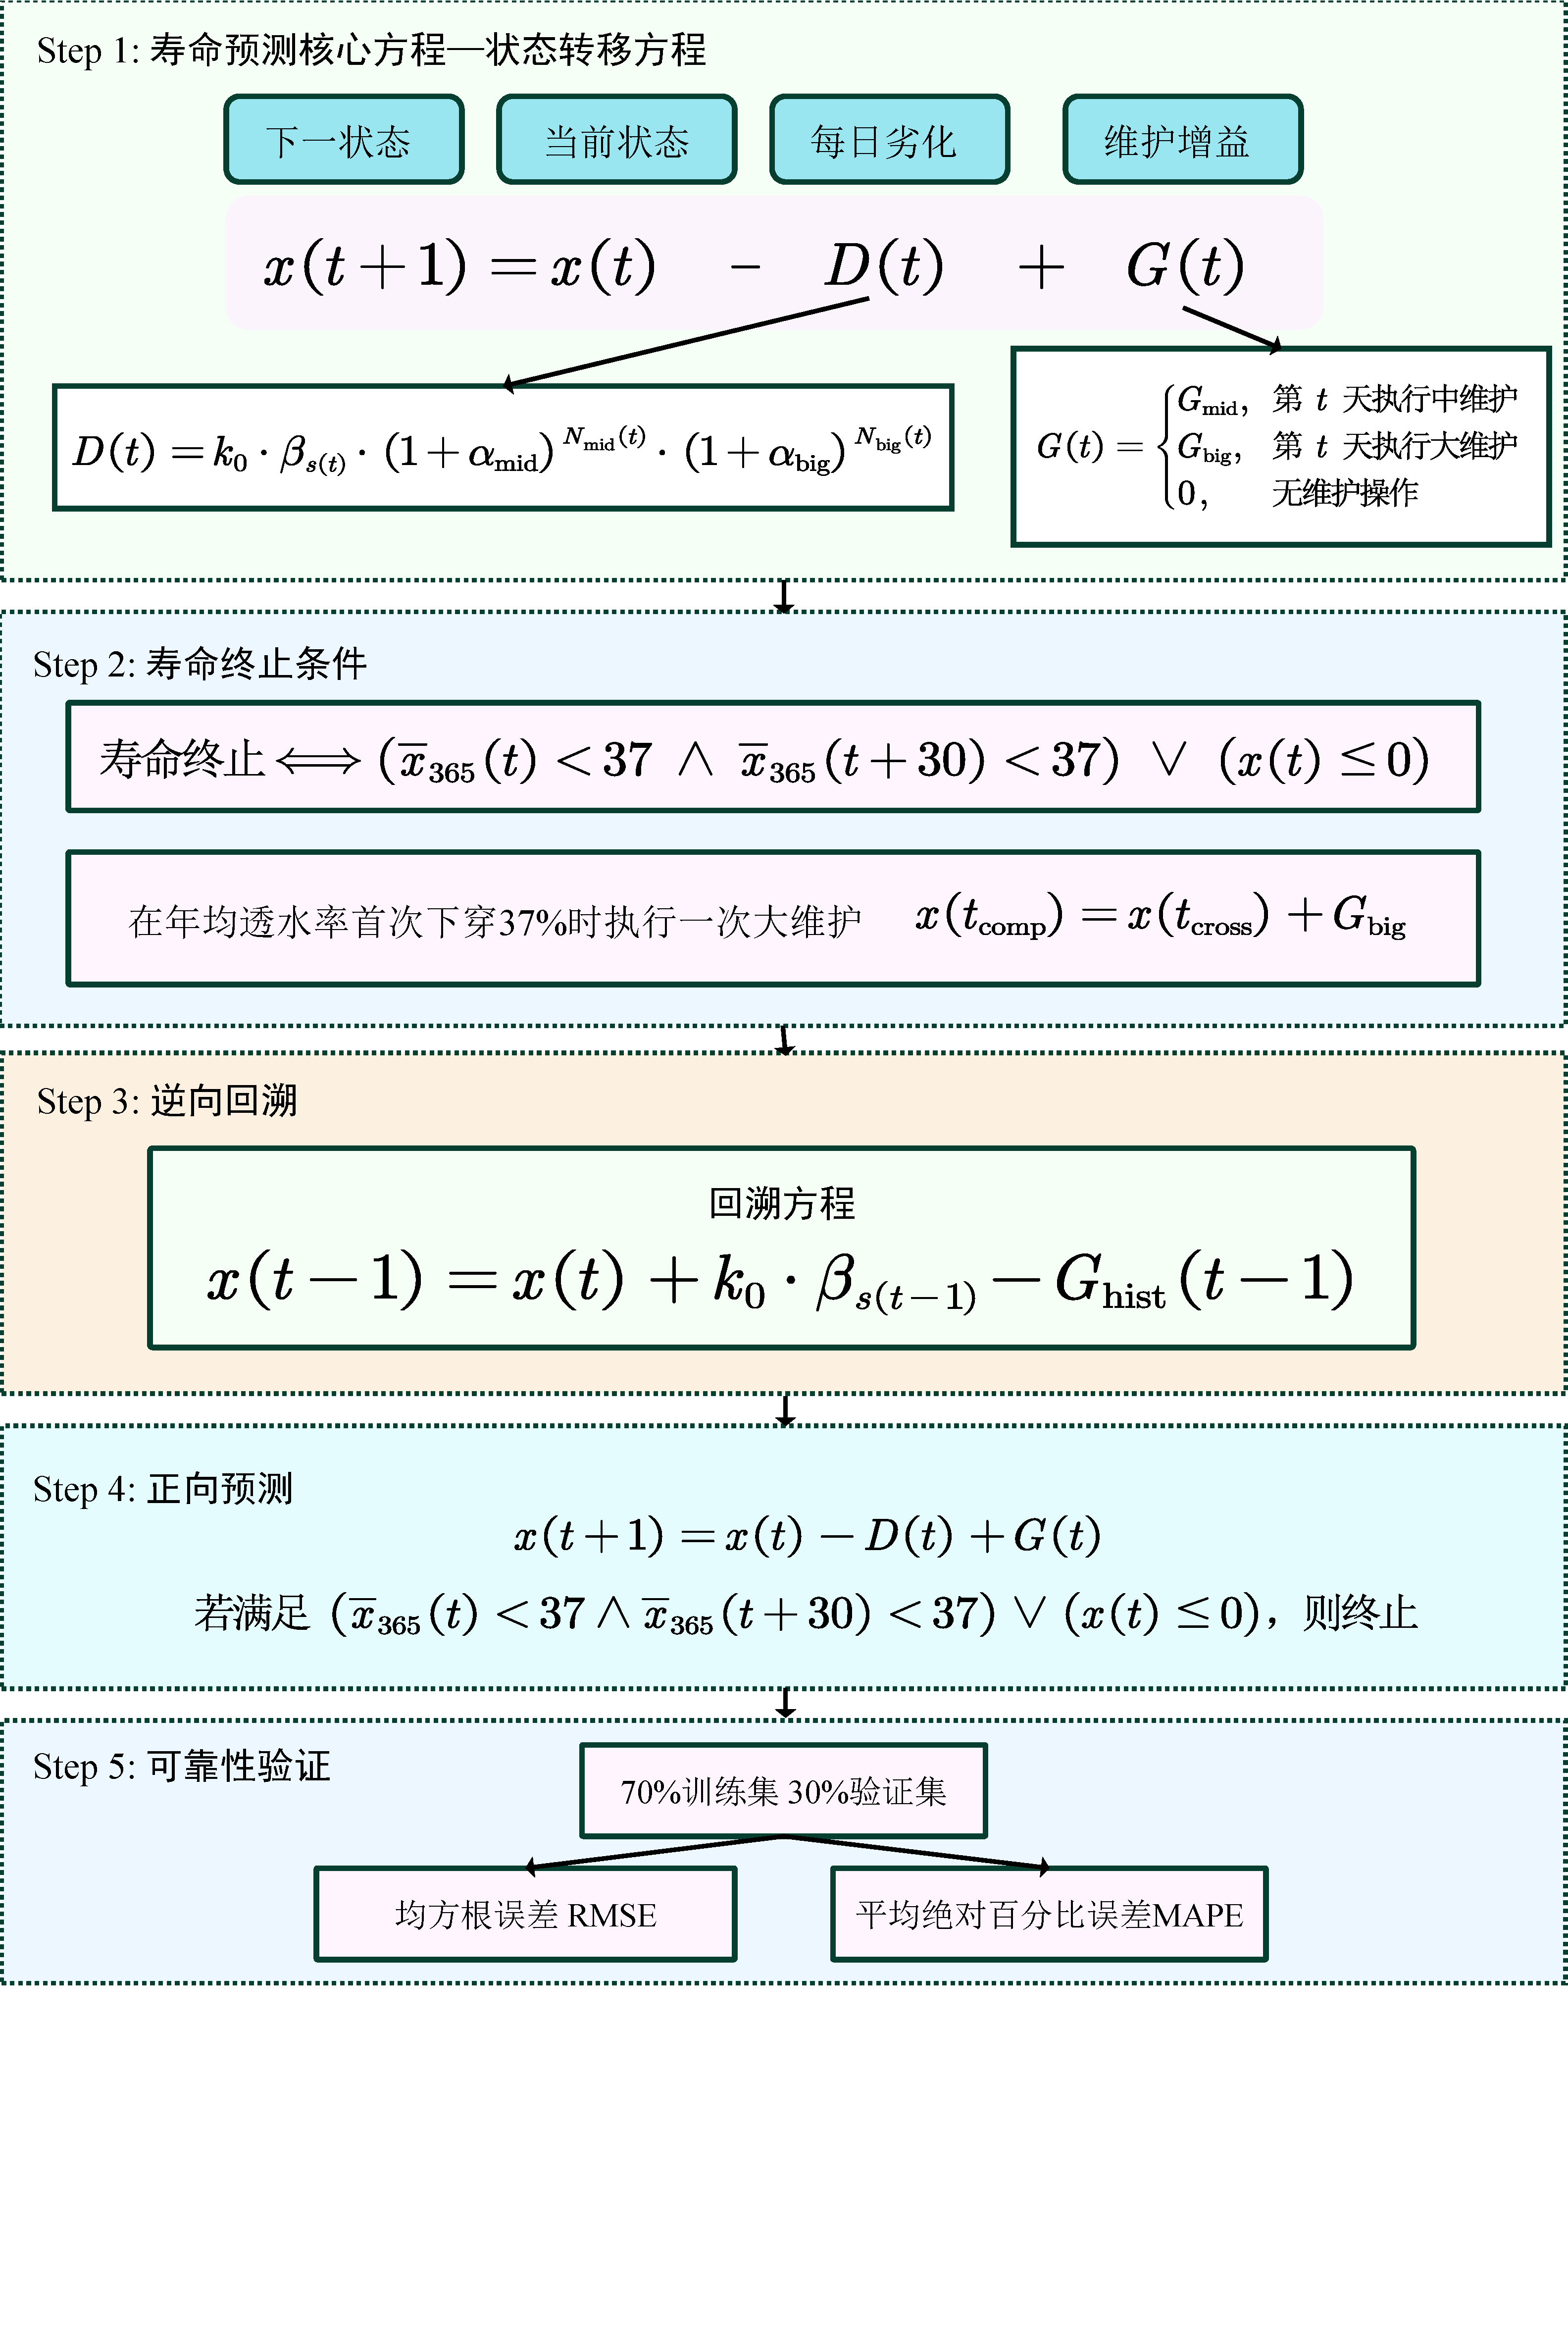
\includegraphics[
%	width=0.63\textwidth,
%	trim=0cm 12cm 0cm 0cm, 
%	clip
%	]{figures/问题二分析.pdf}
%	\caption{问题二分析流程图}
%	\label{fig:问题二分析}
%\end{figure}


本问的难点在于每日 0:00 无法获知当日真实的小区负载与光伏发电功率，需先预测再优化，且预测与实际的偏差会在运行过程中逐步暴露。

预测环节中，负载侧基于小区用电早晚高峰、工作日与周末差异、全年缓慢升降三类稳定规律，通过 MSTL 分解为趋势、日周期、周周期与残差四部分，若残差存在显著自相关性则补充 AR (p) 模型，将其进一步分解为短期自相关部分与白噪声；光伏侧将发电特性拆分为由太阳运行决定的季节晴空强度与由天气决定的日透射率，对日透射率序列采用 AR (p) 开展日尺度滚动预测，乘性结构无法解释的日内短时波动残差参照负载残差的逻辑处理，同时施加非负与夜间归零的物理约束。针对初始阶段无历史数据导致模型无法启动的问题，以附件 1 的典型负载与光伏曲线为先验模板，与逐步积累的近期实际数据加权混合，随时间推移逐步降低先验模板的参考比重，待历史数据足以支撑周周期与晴空包络估计后，完全切换为正式预测模型。此外考虑到预测偏差的代价不对称 —— 预测偏少会触发 5 倍电价的紧急购电、代价远高于预测偏多，故按历史净负荷正向误差的分位数构造风险备用量叠加到预测值上，为缺电侧预留余量；缺口实际出现时调用储能还是紧急购电，由日内优化按成本决策。

优化沿用第一问框架，仅调整日内滚动目标函数：0:00 后计划购电费已锁定，只需最小化紧急购电费、跨日按正常电价计的虚拟购电费，并附加极小循环惩罚以抑制同时充放电。

\subsection{问题三分析}

首先处理预报粒度与模型时段的匹配问题，附件 3 给出的是每小时的预报，而模型以 10 分钟为时段。于是我们将整点预报线性插值到 10 分钟时段。除此之外，问题三的优化结构相对问题二变化不大，只需要把购电调整量，分解为向上与向下两部分即可：$P^{\mathrm{buy}}_{k,t}=P^{\mathrm{buy}}_{k-1,t}+U^{+}_{k,t}-U^{-}_{k,t}$，分别按 $1.5\lambda_t U^{+}_{k,t}\Delta t$ 与 $0.5\lambda_t U^{-}_{k,t}\Delta t$ 分别计入追加和违约费用。为判断是否有必要引入其他时刻的预报，我们构造了光伏发电功率的动态非对称风险带。由于预测偏高易触发高价的紧急购电，风险带的危险侧容许宽度更窄。随后，我们通过计算预测值偏离带状区域的越界量来量化各时段的“风险集中度”，并据此筛选出需要增加额外预报的候选时点。


\subsection{问题四分析}

在电价是波动的情况下，由于电价同样具有显著的日周期与周周期特征，我们沿用问题二与问题三中的MSTL结合AR模型，构建电价的48小时滚动预测模块。在优化部分，问题四完全继承前两问的建模，包括动态非对称风险机制、储能设备物理约束等。仅在决策时将目标函数中的结算电价替换为预测电价，最后计算购电费时切换成真实电价。在判断是否引入其他预报时点时，由于问题三的信息差主要来自光伏发电功率，而在问题四波动电价的情况下，电价预测误差会导致产生独立于光伏的经济损失，所以我们定义包含光伏和电价的联合经济风险，作为其他预报时点的判定。

%%%%%%%%%%%%%%%%%%%%%%%%%%%%%%%%%%%%%%%%%%%%%%%%%%%%%%%%%%%%% 

\section{模型假设}

\begin{enumerate}[label=\arabic*.]
	\item 附件1给出的电价、小区负载与光伏发电预测功率在对应10分钟时段内保持恒定；
	\item 微网只允许向外部电网购电，不允许向外部电网反送电；
	\item 弃电仅来源于光伏发电的富余部分，不丢弃外网购电与储能设备放电；
	\item 储能设备充、放电效率恒定为0.9，不随储电量、温度与设备老化而变化，且忽略自放电与待机损耗；
	\item 外部电网供电能力充足，紧急购电与购电方案调整均可在对应时段瞬时完成，不考虑最小调整粒度与供应上限；
	\item 忽略微网内部线路与变压器损耗，功率平衡在并网点处成立；
	\item 不考虑设备故障、检修与寿命衰减对运行策略的影响；
	\item 负荷与光伏预测误差的统计特性在短期内保持平稳，未来时段的误差分布可由近期同日型历史样本近似表征；
\end{enumerate}

%%%%%%%%%%%%%%%%%%%%%%%%%%%%%%%%%%%%%%%%%%%%%%%%%%%%%%%%%%%%% 
\vspace*{-7pt}
\section{符号说明}
\vspace*{-7pt}
\begin{table}[h!]
	\centering
	\renewcommand{\arraystretch}{1.2}
%	\small
	\setlength{\tabcolsep}{5pt}
%	\caption{主要符号说明}
	\label{tab:符号说明}
	\begin{tabular}{lcc}
		\toprule[1.5pt]
		\textbf{符号} & \textbf{说明} & \textbf{单位} \\
		\midrule
		\rowcolor{LightBlue}
		$d, t, h, k$ & 天索引、10分钟时段索引、小时索引、预报发布阶段 & -- \\
		$P^{\mathrm{L}}_{d,t}, P^{\mathrm{PV}}_{d,t}, P^{\mathrm{net}}_{d,t}$ & 第 $d$ 天第 $t$ 时段的实际负荷、光伏、净负荷功率 & kW \\
		\rowcolor{LightBlue}
		$\hat{P}^{\mathrm{L}}_{d,t}, \hat{P}^{\mathrm{PV}}_{d,t}, \hat{P}^{\mathrm{net}}_{d,t}$ & 对应上述物理量的预测值 & kW \\
		$e^{\mathrm{net}}_{d,t}$ & 净负荷预测误差（实际值减预测值） & kW \\
		\rowcolor{LightBlue}
		$E^{\mathrm{buy}}_{d,t}, E^{\mathrm{ch}}_{d,t}, E^{\mathrm{dis}}_{d,t}$ & 第 $d$ 天第 $t$ 时段的计划购电量、充电量、放电量 & kWh \\
		$E^{\mathrm{emg}}_{d,t}, E^{\mathrm{sur}}_{d,t}$ & 第 $d$ 天第 $t$ 时段的紧急购电量、富余电量 & kWh \\
		\rowcolor{LightBlue}
		$\lambda_t, \hat{\lambda}_t$ & 第 $t$ 时段的真实波动电价与预测电价 & 元/kWh \\
		$S_t, S_{\min}, S_{\max}$ & 第 $t$ 时段末储电量及其安全运行下限、上限 & kWh \\
		\rowcolor{LightBlue}
		$P_{\max}, \eta_c, \eta_d$ & 储能设备最大充放电功率、充电效率、放电效率 & kW, --, -- \\
		$b^+_t, b^-_t$ & 动态非对称风险带的上侧（危险）与下侧（安全）容许宽度 & kW \\
		\rowcolor{LightBlue}
		$\Delta_t$ & 光伏预测危险高估越界量 & kW \\
		$B_{d,h}$ & 基线方案下第 $d$ 天第 $h$ 小时的购电量 & kWh \\
		\rowcolor{LightBlue}
		$G^{\mathrm{PV}}_{d,t}$ & 季节晴空强度（近似晴空下当天各时段本应发的电功率） & kW \\
		$R^{\mathrm{risk}}_{d,t}, \rho$ & 时段风险备用量、风险强度系数 & kW, -- \\
		\rowcolor{LightBlue}
		$\alpha_{d,t}, \beta_{d,t}, \tau_{d,t}$ & 动态非对称风险权重（正/负向）、最优分位水平 & --, --, -- \\
		$c^+_t, c^-_t$ & 单位正/负向误差的边际补救代价 & 元/kWh \\
		\rowcolor{LightBlue}
		$C_{\mathrm{total}}$ & 全年累计总购电费用 & 元 \\
		\bottomrule[1.5pt]
	\end{tabular}
\end{table}

%%%%%%%%%%%%%%%%%%%%%%%%%%%%%%%%%%%%%%%%%%%%%%%%%%%%%%%%%%%%% 

\section{问题一的模型建立与求解}

问题一要求在电价、小区负载与光伏发电预测功率均已知的确定性条件下，制定微网单日（144 个 10 分钟时段）的计划购电策略与储能设备充放电方案，使全天购电费用最小。由于目标函数与全部约束均可表示为决策变量的线性表达式，我们将其建立为线性规划（LP）模型，并调用线性规划求解器求得全局最优解\upcite{1}。

\subsection{单日购电与储能调度优化模型}

\subsubsection{决策变量与参数}

取第 $t$ 个 10 分钟时段（$t=1,2,\dots,144$，时段长度 $\Delta t=1/6$ h）的外网购电功率 $P^{\mathrm{buy}}_t$、储能设备充电功率 $P^{\mathrm{ch}}_t$、储能设备放电功率 $P^{\mathrm{dis}}_t$、富余功率 $P^{\mathrm{curt}}_t$ 以及时段末储电量 $S_t$ 为决策变量，对应电量由 $E_t=P_t\Delta t$ 换算。已知参数为：电价 $c_t$、小区负载功率 $P^{\mathrm{L}}_t$、光伏预测功率 $P^{\mathrm{PV}}_t$、充放电效率 $\eta=0.9$、最大充放电功率 $P_{\max}=5000$ kW、安全电量区间 $[S_{\min},S_{\max}]=[1200,10800]$ kWh、初始储电量 $S_0=6000$ kWh。

\subsubsection{目标函数}

以全天购电费用最小为目标：
\begin{equation}
	\min \sum_{t=1}^{144} c_t P^{\mathrm{buy}}_t \Delta t.
	\label{eq:q1obj}
\end{equation}

\subsubsection{约束条件}

\begin{enumerate}[label=(\arabic*),leftmargin=40pt]
	
	\item 电力收支平衡：光伏发电、外网购电与储能设备放电之和，等于小区负载、储能设备充电与弃电之和：
	\(
		P^{\mathrm{PV}}_t + P^{\mathrm{buy}}_t + P^{\mathrm{dis}}_t
		=
		P^{\mathrm{L}}_t + P^{\mathrm{ch}}_t + P^{\mathrm{curt}}_t,\quad \forall t.
		\label{eq:q1balance}
	\)
	
	\item 弃电仅来自光伏富余，不得超过该时段光伏预测功率：
	\(
		0 \le P^{\mathrm{curt}}_t \le P^{\mathrm{PV}}_t,\quad \forall t.
		\label{eq:q1curt}
	\)
	
	\item 储能设备电量状态转移：充电按效率 $\eta$ 折算存入，放电按 $1/\eta$ 折算消耗内部电量：
	\(
		S_t = S_{t-1} + \eta P^{\mathrm{ch}}_t \Delta t - \dfrac{P^{\mathrm{dis}}_t \Delta t}{\eta},\quad \forall t.
		\label{eq:q1soc}
	\)
	
	\item 安全电量区间，避免过度充电或过度放电：
	\(
		S_{\min} \le S_t \le S_{\max},\quad \forall t.
		\label{eq:q1socbound}
	\)
	
	\item 充放电功率上限：
	\(
		0 \le P^{\mathrm{ch}}_t \le P_{\max},\quad
		0 \le P^{\mathrm{dis}}_t \le P_{\max},\quad \forall t.
		\label{eq:q1pbound}
	\)
	
	\item 外网购电非负：
	\(
		P^{\mathrm{buy}}_t \ge 0,\quad \forall t.
		\label{eq:q1buynonneg}
	\)
	
	\item 单日首末储电量相同，并取附录 1 给出的初始电量：
	\(
		S_0 = S_{144} = 6000.
		\label{eq:q1socend}
	\)
	
\end{enumerate}

目标函数与所有约束均为决策变量的线性表达式，构成一个线性规划问题，可由单纯形法或内点法求得全局最优解。

\subsection{模型求解与结果分析}

调用 SciPy 优化模块中的 \texttt{linprog} 函数（HiGHS 求解器）对上述线性规划进行求解。下面从功率平衡、购电策略、储能调度与功率去向四个角度展示并验证求解结果。

\begin{lstlisting}[language=Python]
c = np.zeros(4 * T); c[0::4] = pri * dt  # 目标系数: 仅购电按电价计费
bounds = [b for t in range(T) for b in ((0, None), (0, Pmax), (0, Pmax), (0, pv[t]))]
# 购电/充电/放电/弃电的上下界
res = linprog(c, A_ub=A_ub, b_ub=b_ub, A_eq=A_eq, b_eq=b_eq, bounds=bounds, method='highs')
# HiGHS自动选用单纯形法或内点法求全局最优
pbuy, pch, pdis, pw = res.x.reshape(T, 4).T  # 拆回购电/充电/放电/弃电四条功率曲线
\end{lstlisting}

\vspace*{-30pt}
% 图文件：figures/第一问微网功率平衡.png
\begin{figure}[H]
	\centering
	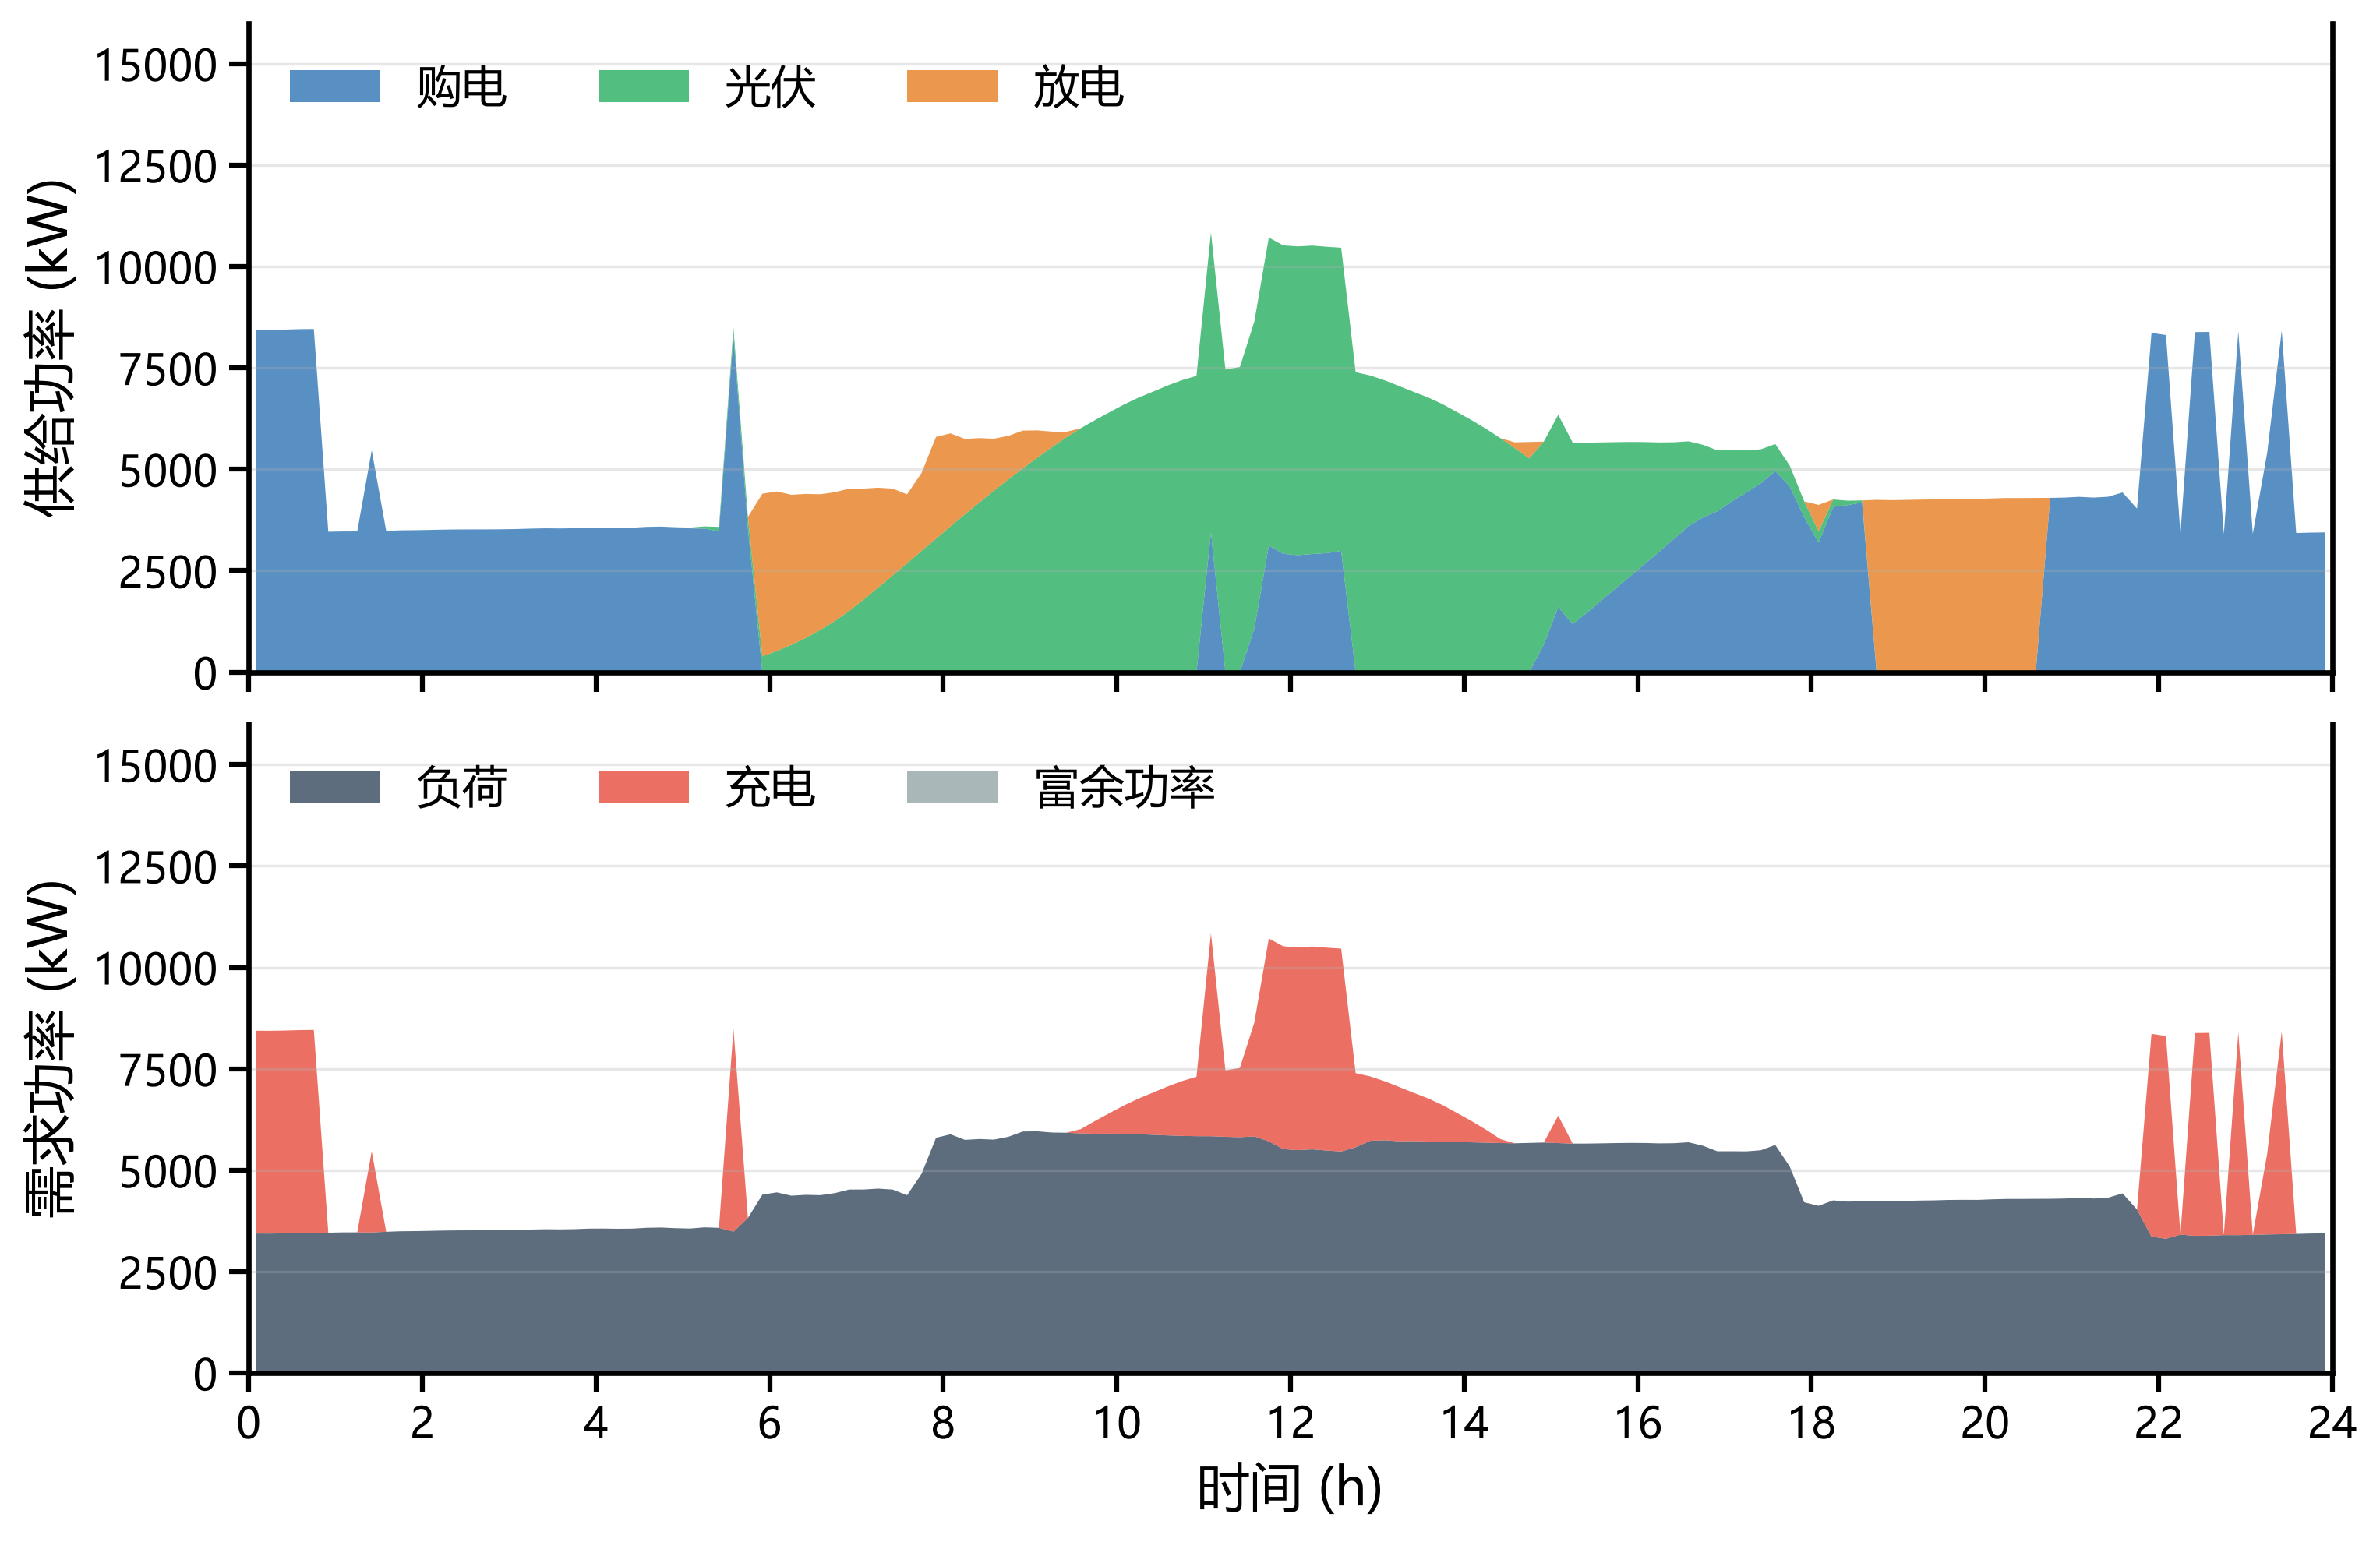
\includegraphics[width=.7\textwidth]{figures/第一问微网功率平衡.png}
	\caption{问题一微网功率平衡：供给侧与需求侧逐时段对照}
	\label{fig:q1balance}
\end{figure}

图~\ref{fig:q1balance} 将功率平衡约束 \ref{eq:q1balance} 的供给侧（购电、光伏、放电）与需求侧（负载、充电、富余功率）逐时段堆叠对照。午间光伏出力高于负载时，富余部分可被储能设备充电吸收，夜间与早晚高峰时段则由购电与放电补足负载。

% 图文件：figures/第一问计划购电功率与电价分时对照.png
\begin{figure}[H]
	\centering
	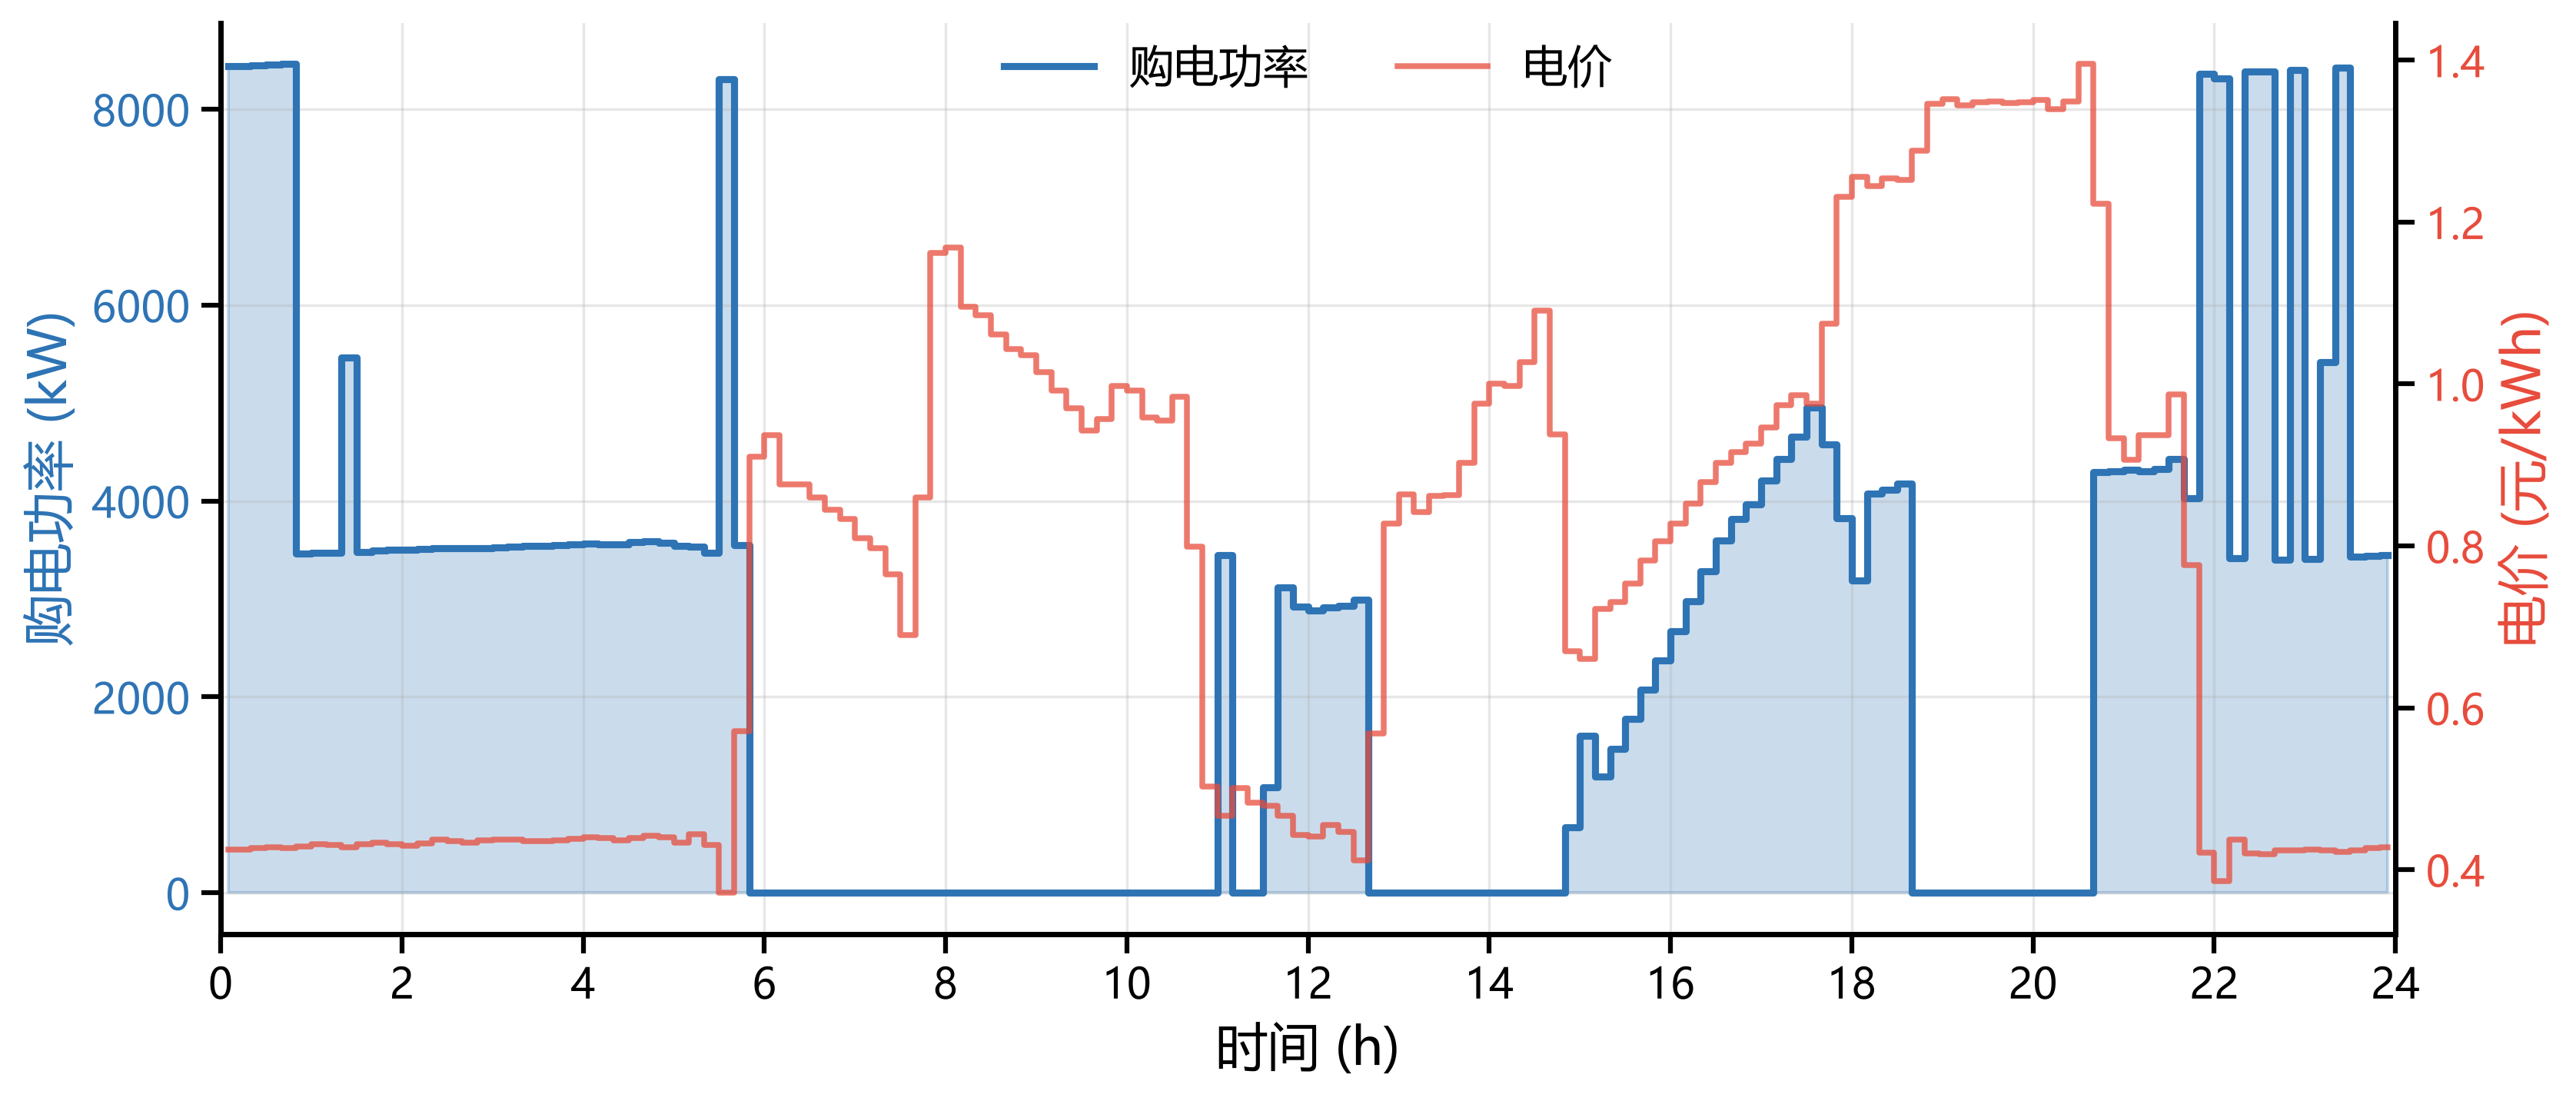
\includegraphics[width=.7\textwidth]{figures/第一问计划购电功率与电价分时对照.png}
	\caption{问题一计划购电功率与电价分时对照}
	\label{fig:q1buyprice}
\end{figure}

由图~\ref{fig:q1buyprice} 可以看出，最优购电策略呈现明显的“低谷多买、高峰不买”特征：购电集中于凌晨与夜间电价低谷，在满足小区负载的同时以满功率 5000 kW 为储能设备充电；早高峰与晚高峰购电功率降为 0；午间除 11:40--12:40 因储能设备尚未充满且电价较低而少量购电充电外，其余时段购电为 0。

% 图文件：figures/第一问储能充放电.png
\begin{figure}[H]
	\centering
	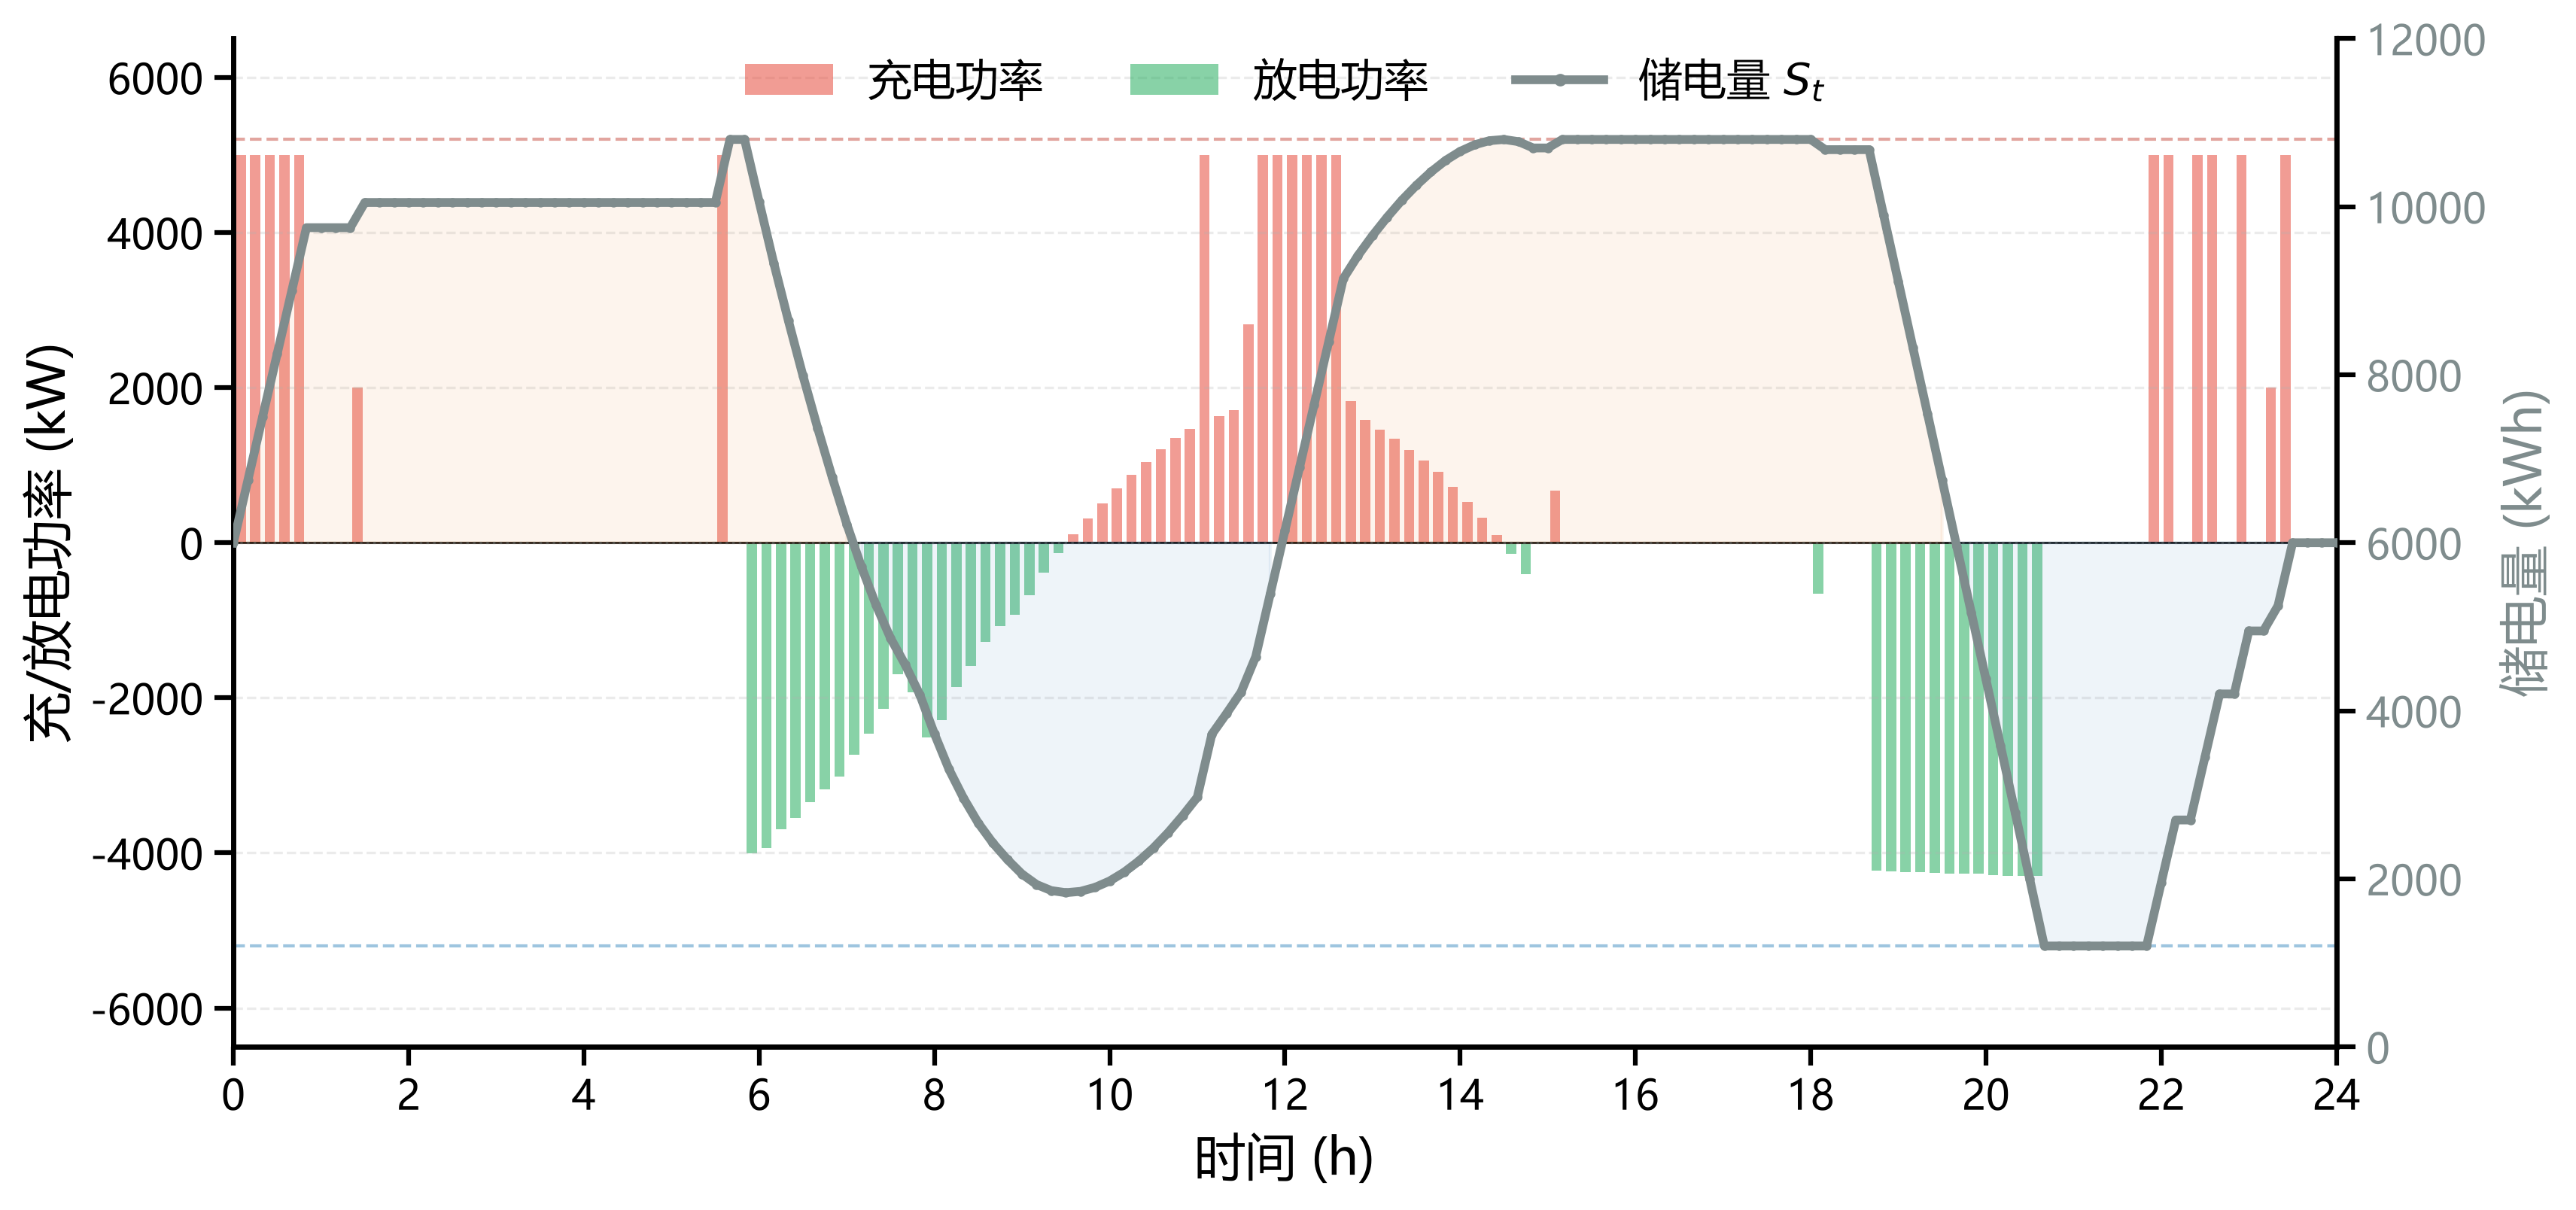
\includegraphics[width=.7\textwidth]{figures/第一问储能充放电.png}
	\caption{问题一储能设备充放电功率与储电量轨迹}
	\label{fig:q1chdis}
\end{figure}

由图~\ref{fig:q1chdis}，储电量 $S_t$ 在 1200--10800 kWh 上下限之间波动，并于 24:00 回落至 6000 kWh，满足约束 \ref{eq:q1socend}；储电量在午间与午后多次触及上限、在晚高峰触及下限，表明储能设备容量在本题电价结构下被充分利用；充电主要集中于夜间、中午，分别对应夜间电价低集中购电、中午光伏发电富余。

% 图文件：figures/第一问计划购电的功率去向.png 与 figures/第一问光伏发电的功率去向.png
\begin{figure}[H]
	\centering
	\subcaptionbox{计划购电功率的去向\label{fig:q1flowbuy}}%
	{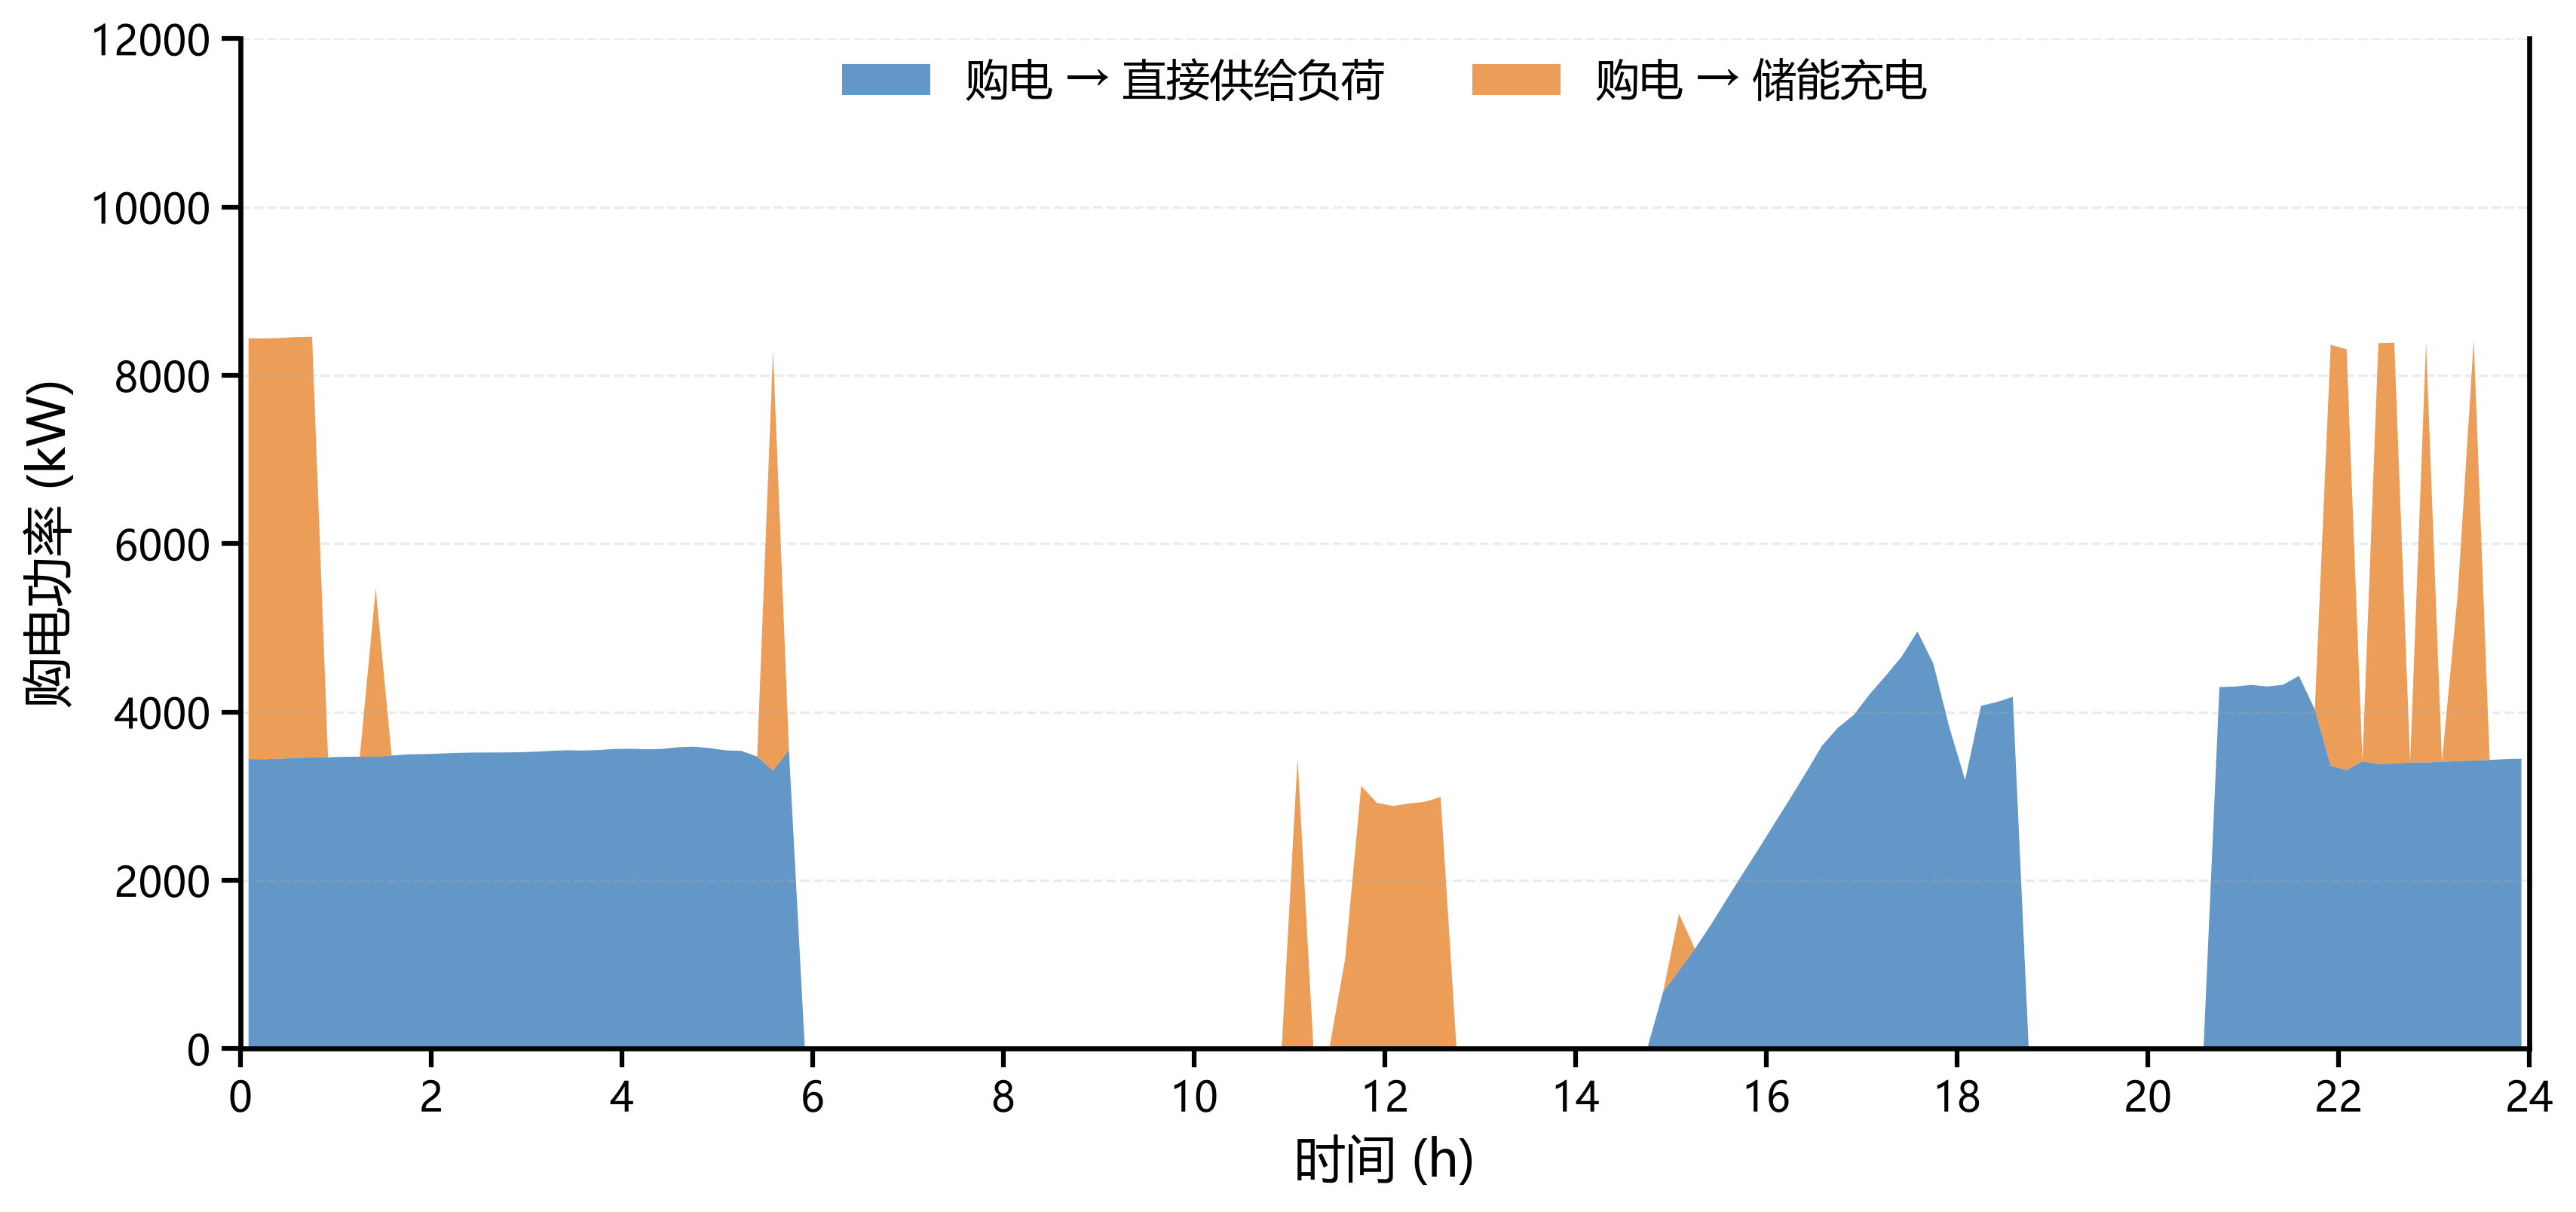
\includegraphics[width=.48\textwidth]{figures/第一问计划购电的功率去向.png}}%
	\hfill
	\subcaptionbox{光伏发电功率的去向\label{fig:q1flowpv}}%
	{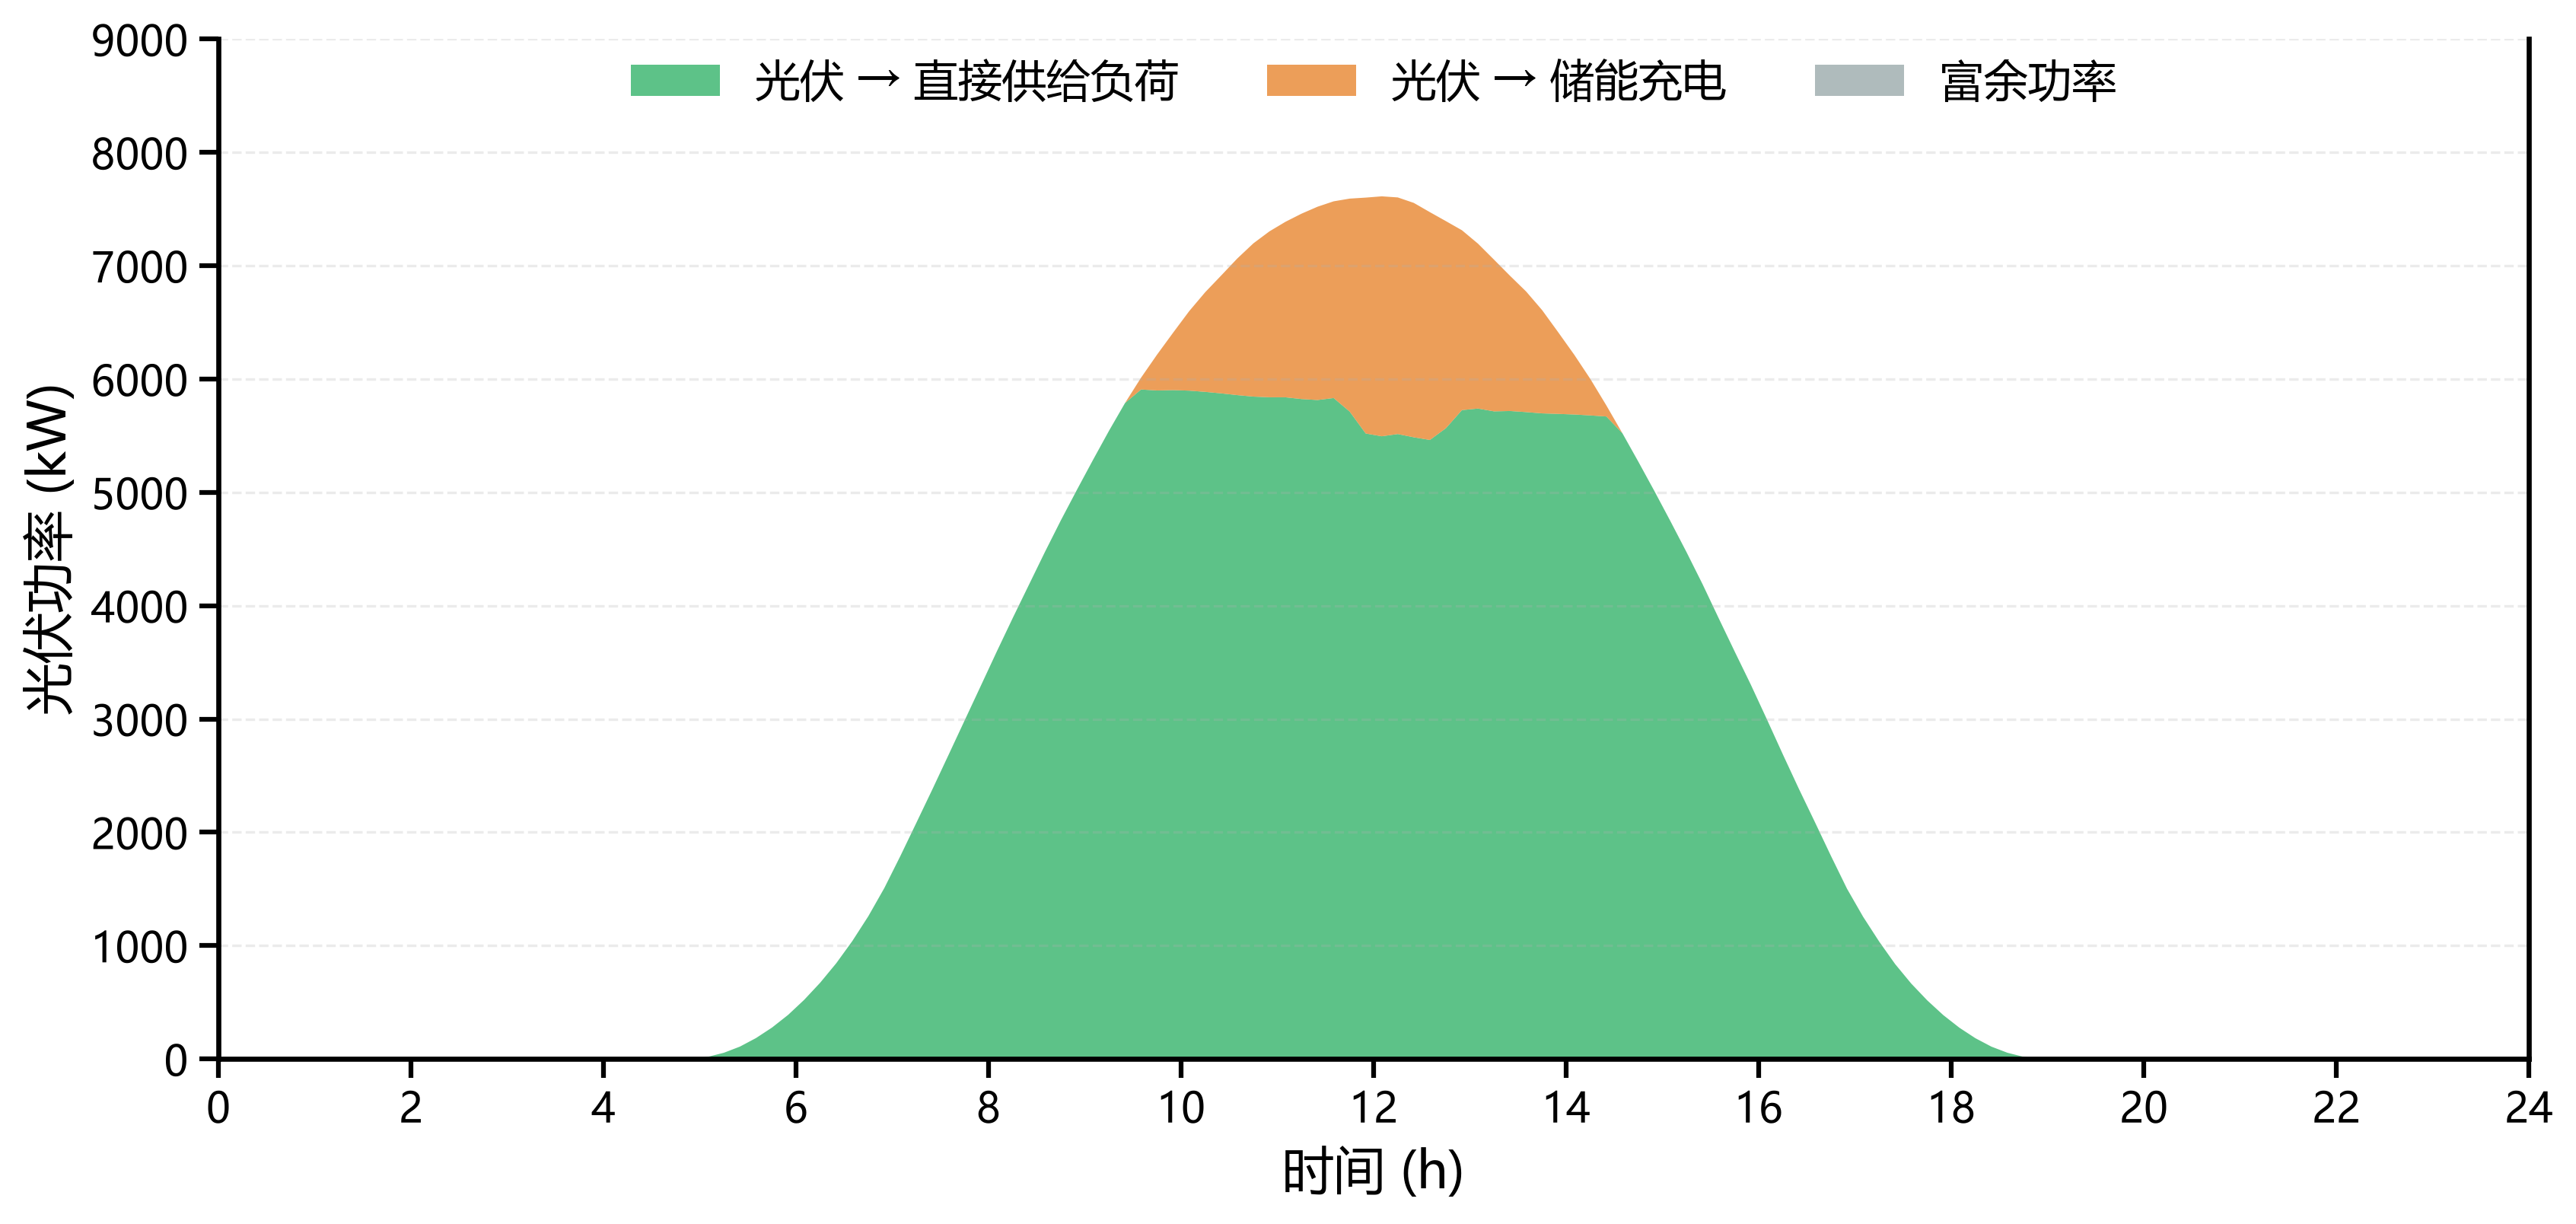
\includegraphics[width=.48\textwidth]{figures/第一问光伏发电的功率去向.png}}
	\caption{问题一计划购电与光伏发电的功率去向}
	\label{fig:q1flow}
\end{figure}

图~\ref{fig:q1flow} 从能量去向角度进一步验证调度结构：全天购电 59483 kWh 中 75.6\% 直接供给负荷、24.4\% 用于储能设备充电；全天光伏 55483 kWh 中 88.7\% 直接供给负荷、11.3\% 存入储能设备、富余功率为 0。购电、光伏充电合计 20741 kWh。具体求解结果如下：

\begin{table}[H]
	\centering
	\renewcommand{\arraystretch}{1.2}
	\setlength{\tabcolsep}{15pt}
	\footnotesize
	\caption{微网在指定时间段的购电量及全天的购电量和购电费}
	\label{tab:q1buy}
	\begin{tabular}{|c|c|c|c|c|c|}
		\hline
		时间段 & 购电量 & 时间段 & 购电量 & 时间段 & 购电量 \\ \hline
		10:00-10:10 & 0.0000 & 12:00-12:10 & 486.4029 & 14:00-14:10 & 0.0000 \\ \hline
		16:00-16:10 & 394.9315 & 18:00-18:10 & 636.9826 & 20:00-20:10 & 0.0000 \\ \hline
		\multicolumn{2}{|c|}{全天购电量} & 59482.6990 & \multicolumn{2}{c|}{全天购电费} & 35126.9500 \\ \hline
	\end{tabular}
\end{table}

\begin{table}[H]
	\centering
	\renewcommand{\arraystretch}{1.2}
	\setlength{\tabcolsep}{15pt}
	\footnotesize
	\caption{储能设备在指定时间段的充放电量及 0:00 和 24:00 的储电量}
	\label{tab:q1ess}
	\begin{tabular}{|c|c|c|c|c|c|}
		\hline
		时间段 & 充电量 & 放电量 & 时间段 & 充电量 & 放电量 \\ \hline
		0:00-4:00 & 4500.0000 & 0.0000 & 4:00-8:00 & 833.3333 & 6365.8412 \\ \hline
		8:00-12:00 & 4787.9643 & 1702.9970 & 12:00-16:00 & 5286.0352 & 91.1014 \\ \hline
		16:00-20:00 & 0.0000 & 5780.1319 & 20:00-24:00 & 5333.3333 & 2859.8681 \\ \hline
		\multicolumn{2}{|c|}{0:00 储电量} & 6000.0000 & \multicolumn{2}{c|}{24:00 储电量} & 6000.0000 \\ \hline
	\end{tabular}
\end{table}

%由表~\ref{tab:q1buy} 可见，10:00--10:10、14:00--14:10 与 20:00--20:10 三个时段购电量为 0，分别对应光伏富余期与晚高峰放电期；12:00--12:10、16:00--16:10 与 18:00--18:10 仍需少量购电，用于弥补光伏出力下降与储能放电功率上限之间的缺口。由表~\ref{tab:q1ess} 可见，充电主要发生在 0:00--4:00、12:00--16:00 与 20:00--24:00 的电价低谷或光伏富余期，放电主要发生在 4:00--8:00 与 16:00--20:00 的电价高峰，充放电量在能量守恒与效率折算下恰好使首末储电量同为 6000 kWh，验证了约束 (\ref{eq:q1socend}) 的有效性。

%%%%%%%%%%%%%%%%%%%%%%%%%%%%%%%%%%%%%%%%%%%%%%%%%%%%%%%%%%%%% 

\section{问题二的模型建立和求解}

问题二须在实际值未知时确定全天购电策略，预测偏差可能触发高价紧急购电。本问建模分为预测与优化两部分：每天 0:00 基于历史数据预测未来 48 h 的负载与光伏发电功率，经非对称风险校准得到校准净负荷；随后确定日前购电计划，并在日内通过局部修正消化实时偏差。其中，前 144 个 10 分钟 时段用于当天日前计划，后 144 个时段用于跨越午夜评估储能设备的未来价值。

\vspace*{-5pt}
\subsection{预测模型}

预测模型分为四个部分，负载预测、光伏发电功率预测、冷启动处理办法、非对称风险校准。

\subsubsection{负载预测}

负载同时具有日内生活规律、工作日与周末差异及全年缓慢升降三类结构。由于每 10 min 一个观测点，一天与一周分别对应144与1008个时段，故采用 MSTL 将负载分解为趋势、日周期、周周期与残差四部分：
\vspace*{-7pt}
\begin{equation}
	P^{\mathrm{L}}_{t}=T^{\mathrm{L}}_{t}+S^{\mathrm{L}}_{144,t}+S^{\mathrm{L}}_{1008,t}+R^{\mathrm{L}}_{t},
	\label{eq:q2mstl}
\end{equation}
其中 $t$ 为 10 min 时段序号（$t=1,2,\dots,144$），$T^{\mathrm{L}}_t$ 为缓慢变化的趋势项，$S^{\mathrm{L}}_{144,t}$ 与 $S^{\mathrm{L}}_{1008,t}$ 分别为周期 144 与 1008 的季节项，对应日周期与周周期，$R^{\mathrm{L}}_t$ 为剔除确定性结构后的残差。MSTL 以局部加权回归依次提取各季节分量与趋势分量，对邻近观测赋予较高权重\upcite{2}：
\begin{equation}
	\min_{\beta}\sum_i w_i(t)\left(y_i-x_i^{\mathrm{T}}\beta\right)^2,
	\label{eq:q2loess}
\end{equation}
其中 $y_i$ 为第 $i$ 个观测点的负载功率，$x_i$ 为该点局部回归的设计向量，$\beta$ 为待估的局部回归系数，$w_i(t)$ 为第 $i$ 个观测在目标时刻 $t$ 处的权重，距 $t$ 越近权重越大。本题仅含一年数据，年周期只有一个完整样本，无法稳定估计，故不另设年季节项，而由趋势项 $T^{\mathrm{L}}_t$ 承担全年升降。若分解残差仍存在显著自相关，则建立 AR($p$)模型：
\vspace*{-7pt}
\begin{equation}
	R^{\mathrm{L}}_{t}=c+\sum_{i=1}^{p}\phi_i R^{\mathrm{L}}_{t-i}+\varepsilon_t,
	\label{eq:q2arL}
\end{equation}
其中 $c$ 为常数项，$\phi_i$ 为第 $i$ 阶自回归系数，$\varepsilon_t$ 为白噪声。该式将残差分解为可预测的短期自相关部分与白噪声，阶数 $p$ 从候选集合 $\{1,2,3,6,12,18,36\}$ 中按滚动预测误差选取。最终负载预测为各分量预测之和：
\begin{equation}
	\hat P^{\mathrm{L}}_{t+h}=\hat T^{\mathrm{L}}_{t+h}+\hat S^{\mathrm{L}}_{144,t+h}+\hat S^{\mathrm{L}}_{1008,t+h}+\hat R^{\mathrm{L}}_{t+h},
	\label{eq:q2loadpred}
\end{equation}
其中 $h$ 为预测步长（以 10 min 时段计），带帽符号表示对应分量的预测值；趋势项以末端局部趋势外推，季节项按相同相位延拓，残差项由自回归模型递推。为控制计算量，我们采用“低频完整分解、高频轻量更新”策略：由于日、周用电规律数日内几乎不变，两次完整拟合间直接复用其周期模板；针对逐日漂移的整体水平，提取最近 3 天数据扣除周期模板得到去季节化序列，拟合直线外推趋势（斜率限幅于 $\pm5$ kW/时段以防发散）；并每日更新残差自回归的递推起点。该机制使 MSTL 计算量降至原来的 $\frac{1}{7}$，在保证精度的同时显著提升求解效率。

\subsubsection{光伏发电功率预测}

光伏功率的日内形状与季节幅值由太阳位置决定，具有确定性；当日发电水平则主要受云量等天气因素衰减。据此将光伏功率表示为季节晴空强度与日透射率的乘积加残差：
\begin{equation}
	P^{\mathrm{PV}}_{d,t}=G^{\mathrm{PV}}_{d,t}\,\kappa_d+R^{\mathrm{PV}}_{d,t},\qquad 0\le\kappa_d\le 1,
	\label{eq:q2pv2term}
\end{equation}
其中 $d$ 为日期序号，$t$ 为时段序号，$G^{\mathrm{PV}}_{d,t}$ 为季节晴空强度，表示近似晴空条件下,当天第 $t$ 时段光伏系统能够转换的最大电功率。$\kappa_d$ 为日透射率，表示当天实际发电量占晴空潜在发电量的比例；$R^{\mathrm{PV}}_{d,t}$ 为乘性结构未能解释的短时残差。晴空强度由滚动历史窗口内同一时刻光伏功率的高分位数估计并平滑得到：
\begin{equation}
	\tilde G^{\mathrm{PV}}_{d,t}=Q_{\alpha}\!\left(\left\{P^{\mathrm{PV}}_{j,t}: j\in W_d\right\}\right),\quad \alpha=0.93,
	\label{eq:q2clear}
\end{equation}
其中 $Q_\alpha(\cdot)$ 表示取 $\alpha$ 分位数（$\alpha=0.93$ 为分位水平），$P^{\mathrm{PV}}_{j,t}$ 为历史第 $j$ 天第 $t$ 时段的实际光伏功率，窗口 $W_d$ 取最近 60 天且仅含 $j<d$ 的历史日以保证不引入未来信息，$\tilde G^{\mathrm{PV}}_{d,t}$ 为平滑前的晴空强度估计，沿日内时间轴平滑后记为 $G^{\mathrm{PV}}_{d,t}$。日透射率定义为
\begin{equation}
	\tilde\kappa_d=\dfrac{\sum_{t=1}^{144}P^{\mathrm{PV}}_{d,t}\Delta t}{\sum_{t=1}^{144}G^{\mathrm{PV}}_{d,t}\Delta t},\qquad
	\kappa_d=\min\{1,\max\{0,\tilde\kappa_d\}\},
	\label{eq:q2kappa}
\end{equation}
其中 $\Delta t=\frac{1}{6}$ h 为时段长度，分子与分母分别为第 $d$ 天的实际发电量与晴空潜在发电量，$\tilde\kappa_d$ 为未截断的透射率估计，$\kappa_d$ 为截断到 $[0,1]$ 后的日透射率。相邻天气过程具有持续性，故对日透射率序列建立 AR($p$) 模型进行日滚动预测\upcite{3}：
\begin{equation}
	\kappa_d=c+\sum_{i=1}^{p}\phi_i\kappa_{d-i}+u_d,
	\label{eq:q2kappaAR}
\end{equation}
其中 $c$ 为常数项，$\phi_i$ 为自回归系数，$u_d$ 为白噪声。由该式得到预测值 $\hat\kappa_d$，阶数 $p$ 从候选集合 $\{1,2,3,5,7\}$ 中选取。结构残差 $R^{\mathrm{PV}}_{d,t}=P^{\mathrm{PV}}_{d,t}-G^{\mathrm{PV}}_{d,t}\kappa_d$ 若自相关显著，同样以自回归模型修正（阶数从 $\{1,2,3,6,12\}$ 中选取）。最终光伏预测重构为
\vspace*{-5pt}
\begin{equation}
	\hat P^{\mathrm{PV}}_{d,t}=G^{\mathrm{PV}}_{d,t}\,\hat\kappa_d+\hat R^{\mathrm{PV}}_{d,t},
	\label{eq:q2pvpred}
\end{equation}
\vspace*{-5pt}
其中 $\hat\kappa_d$ 为日透射率预测值，$\hat R^{\mathrm{PV}}_{d,t}$ 为残差自回归修正项。并施加物理约束：预测值非负，且对历史上稳定无发电的夜间时段直接置零。

\vspace*{-8pt}
\subsubsection{冷启动与一月份预热}

2025 年 1 月 1 日 0:00 尚无历史实际数据，上述模型无法启动。我们以附件 1 的典型负载与光伏曲线作为先验模板，与已积累的近期同一时刻实际值加权融合，使得随着时间推移就越少参考附件1的数据，加权融合表达式如下：
\vspace*{-5pt}
\begin{equation}
	\hat P_{d,t}=w_0(d)\,P^{\mathrm{att1}}_{t}+\sum_{j=1}^{d-1}w_j(d)\,P_{d-j,t},\qquad w_0(d)\downarrow 0,
	\label{eq:q2cold}
\end{equation}
\vspace*{-5pt}
其中 $P^{\mathrm{att1}}_t$ 为附件 1 典型曲线在第 $t$ 时段的取值，$P_{d-j,t}$ 为第 $d-j$ 天第 $t$ 时段的实际值，$w_0(d)$ 与 $w_j(d)$ 分别为先验模板与历史实际值的权重；近期同一时刻实际值按指数衰减加权，先验权重 $w_0(d)$ 随 $d$ 增大单调递减至 0，历史满一周后进一步混入上周曲线数据。历史不足 21 天时以该融合曲线作为预测；达到 21 天后切换至 MSTL 与季节晴空强度的正式模型。\textbf{于是我们规定，下文针对全年的所有求解结果均为从2月1日到年末的求解结果。}

\vspace*{-15pt}
\subsubsection{非对称风险校准}

定义净负荷及其预测与误差：
\vspace*{-5pt}
\begin{equation}
	P^{\mathrm{net}}_{d,t}=P^{\mathrm{L}}_{d,t}-P^{\mathrm{PV}}_{d,t},\quad
	\hat P^{\mathrm{net}}_{d,t}=\hat P^{\mathrm{L}}_{d,t}-\hat P^{\mathrm{PV}}_{d,t},
	\label{eq:q2net}
\end{equation}
\vspace*{-5pt}
其中 $P^{\mathrm{net}}_{d,t}$ 与 $\hat P^{\mathrm{net}}_{d,t}$ 分别为第 $d$ 天第 $t$ 时段的实际净负荷与预测净负荷。相应预测误差为
\vspace*{-5pt}
\begin{equation}
	e^{\mathrm{net}}_{d,t}=\left(P^{\mathrm{L}}_{d,t}-\hat P^{\mathrm{L}}_{d,t}\right)-\left(P^{\mathrm{PV}}_{d,t}-\hat P^{\mathrm{PV}}_{d,t}\right),
	\label{eq:q2enet}
\end{equation}
\vspace*{-5pt}
其中 $e^{\mathrm{net}}_{d,t}$ 为净负荷预测误差，即负载预测误差与光伏发电功率预测误差之差。当 $e^{\mathrm{net}}_{d,t}>0$ 时实际净负荷高于预测，对应负载低估或光伏高估，易触发 5 倍电价的紧急购电；当 $e^{\mathrm{net}}_{d,t}<0$ 时通常仅形成富余，代价较轻，故误差风险具有显著非对称性。

为量化该非对称性，比较单位正向误差的两种补救方式。其一为立即紧急购电，单位正向误差的最小边际补救成本为
\begin{equation}
	c^{+}_{d,t}=\min\left\{5\lambda_t,\ \min_{s\in\mathcal{F}_{d,t}}\frac{\lambda_s}{\eta_c\eta_d}\right\},
	\label{eq:q2cplus}
\end{equation}
\vspace*{-5pt}
其中 $c^{+}_{d,t}$ 为单位正向误差的最小边际补救成本，取立即紧急购电与最优回补两种方案中较便宜的一种；若 $\mathcal{F}_{d,t}=\varnothing$ 则取 $c^{+}_{d,t}=5\lambda_t$。对于负向误差（实际净负荷低于预测），若多余电量无法被储能设备吸收，其单位边际损失即为原计划购电成本 $c^{-}_{d,t}=\lambda_t$。对历史正、负向误差样本分别以指数加权平均，得到单位正向误差边际补救成本与单位负向误差边际损失的滚动估计 $\bar c^{+}_{d,t}$ 与 $\bar c^{-}_{d,t}$。由于非对称损失中起决定作用的是两侧权重的相对比例，不失一般性令 $\beta_{d,t}=1$，并定义动态权重
\vspace*{-5pt}
\begin{equation}
	\alpha_{d,t}=\mathrm{clip}\!\left(\frac{\bar c^{+}_{d,t}}{\max\left\{\bar c^{-}_{d,t},\,\varepsilon_c\right\}},\ \alpha_{\min},\ \alpha_{\max}\right),
	\label{eq:q2alpha}
\end{equation}
%\vspace*{-5pt}
其中 $\varepsilon_c=10^{-4}$，$\mathrm{clip}(\cdot)$ 将权重限制在 $[1,8]$ 内。历史样本不足 5 个时取初值 $\alpha_{d,t}=4$。其合理性可由报童模型解释：相比原计划按 $\lambda_t$ 购电，缺电 1 kWh 需按 5 倍电价紧急购电，额外增加的边际代价 $C_u = 4\lambda_t$；多电 1 kWh 的边际代价 $C_o = \lambda_t$。最优分位水平 $\tau^* = C_u / (C_u + C_o) = 0.8$。在风险校准公式 $\tau_{d,t} = \alpha_{d,t} / (\alpha_{d,t} + \beta_{d,t})$ 中，令 $\beta_{d,t}=1$，为使分位水平匹配 0.8，解得初值 $\alpha_{d,t}=4$\upcite{4}。

在实际运行中，$\alpha_{d,t}$ 由公式 \eqref{eq:q2alpha} 动态计算得出，进而得到时变的分位水平 $\tau_{d,t} = \alpha_{d,t} / (\alpha_{d,t} + 1)$。为了防止极端误差导致 $\tau_{d,t}$ 过大或过小（即过度保守或过度激进），我们将其截断在 $[0.55, 0.88]$ 之间。对最近 28 天同日型历史样本以 0.9 指数衰减加权，取正向净负荷误差的加权 $\tau_{d,t}$ 分位数，再乘以风险强度系数 $\rho$，构造时段风险备用量：
\begin{equation}
	R^{\mathrm{risk}}_{d,t}=\rho\, Q_{\tau}\!\left(\left\{\max\left(e^{\mathrm{net}}_{j,t},\,0\right): j<d\right\}\right),
	\label{eq:q2risk}
\end{equation}
其中 $Q_\tau(\cdot)$ 为加权 $\tau$ 分位数。$\rho$ 反映了系统对预测误差的风险规避程度，由于全年总费用关于 $\rho$ 非凸且非光滑，我们采用“理论指导+滚动回测”确定其值。由于前述报童模型推导的 $\tau^*=0.8$，我们在 $[0.70, 0.90]$ 内以 0.05 为步长进行滚动回测，由图\ref{fig:全年总购电费用随风险强度系数的变化}，全年总费用随 $\rho$ 呈“U 型”变化，并在 $\rho=0.75$ 处达到全局最小，故最终取 $\rho=0.75$。

\begin{figure}[H]
	\centering
	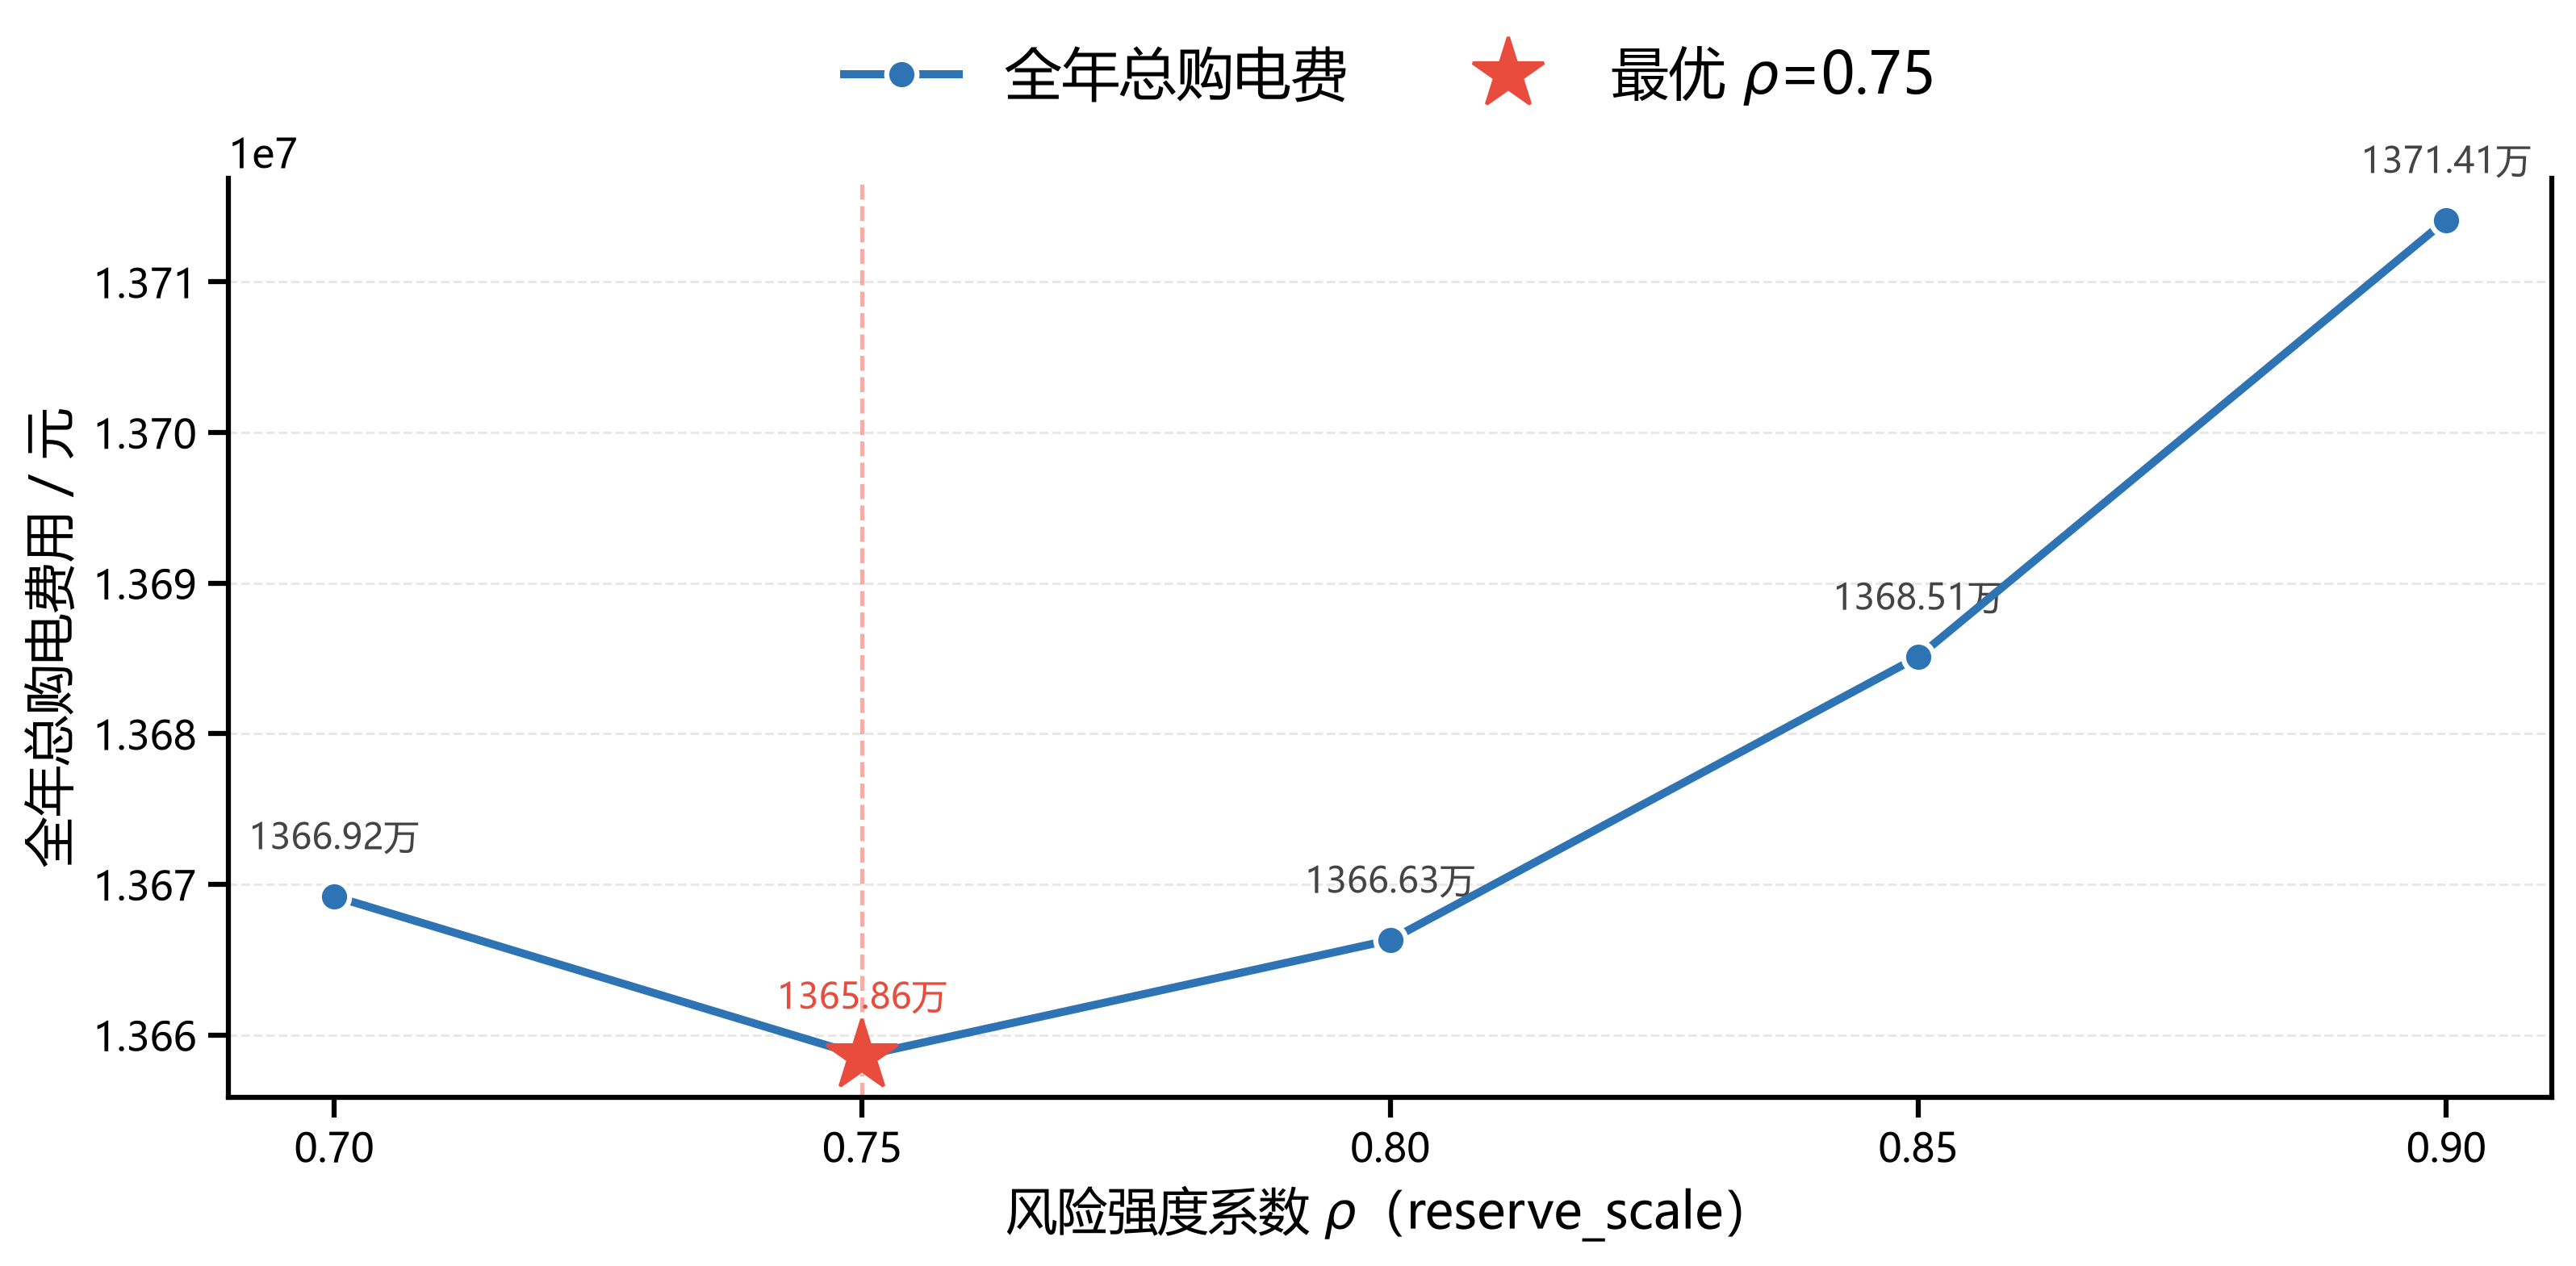
\includegraphics[width=.75\textwidth]{figures/第二问全年总购电费用随风险强度系数的变化.png}
	\caption{全年总购电费用随风险强度系数的变化}
	\label{fig:全年总购电费用随风险强度系数的变化}
\end{figure}

风险校准后的净负荷预测为：$\tilde P^{\mathrm{net}}_{d,t}=\hat P^{\mathrm{net}}_{d,t}+R^{\mathrm{risk}}_{d,t}.$

\subsection{优化模型}

\subsubsection{日前计划购电}

每天 0:00 以风险校准净负荷为需求、以当天 0:00 实际储能状态为初值，求解一次全天线性规划。与第一问相比，问题二的优化模型主要有以下不同：

\begin{enumerate}[label=(\bfseries\arabic*),leftmargin=40pt]

	\item \textbf{目标函数：}
	在计划购电费的基础上，增加日末储能机会价值与循环惩罚两项：
	\begin{equation}
		\min J_d=\sum_{t=1}^{144}\lambda_t P^{\mathrm{buy}}_{d,t}\Delta t
		+\mu\left(S_{d,0}-S_{d,144}\right)
		+\varepsilon\sum_{t=1}^{144}\left(P^{\mathrm{ch,p}}_{d,t}+P^{\mathrm{dis,p}}_{d,t}\right)\Delta t,
		\label{eq:q2dayobj}
	\end{equation}
	其中 $\mu=\eta_d\lambda_{\min}$ 为日末储能机会价值（$\lambda_{\min}$ 为全天最低正常电价），表示日末每保留 1 kWh 电量，次日至少能按放电效率折算出的保守收益，用于防止优化器在日末过度放电；$\varepsilon>0$ 为极小的循环惩罚系数，用于软性抑制无意义的同时充放电。这两项仅影响决策，不计入实际费用。
	
	\item \textbf{功率平衡：}
	需求侧由第一问的已知负载与光伏，替换为风险校准后的预测净负荷 $\tilde P^{\mathrm{net}}_{d,t}$：
	\begin{equation}
		P^{\mathrm{buy}}_{d,t}+P^{\mathrm{dis,p}}_{d,t}=\tilde P^{\mathrm{net}}_{d,t}+P^{\mathrm{ch,p}}_{d,t}+P^{\mathrm{sur,p}}_{d,t}.
		\label{eq:q2daybal}
	\end{equation}
	
	\item \textbf{日内局部修正：}
	计划购电确定后，真实负载与光伏发电功率逐时到达。由于前序时段的预测误差会导致当前真实储电量偏离计划轨迹。因此，设当前时段为 $t$，首先将日前计划充放电功率投影到当前真实储电量与功率上限所允许的可行范围内，得到实际可执行的充、放电功率 $P^{\mathrm{ch}}_{d,t}$ 与 $P^{\mathrm{dis}}_{d,t}$。在此基础上，计算当前时段的实际供需偏差：
	\begin{equation}
		\Delta P_{d,t}=P^{\mathrm{L}}_{d,t}-\left(P^{\mathrm{buy},*}_{d,t}+P^{\mathrm{PV}}_{d,t}+P^{\mathrm{dis}}_{d,t}-P^{\mathrm{ch}}_{d,t}\right),
		\label{eq:q2delta}
	\end{equation}
	若 $\Delta P_{d,t}>0$，表示当前供电不足。为最小化经济损失，按代价递增顺序进行代数修正：首先取消当前时段不必要的计划充电；其次，在最大放电功率与储电量下限允许的范围内增加储能设备放电，代价为消耗储能；若上述调整后仍存在缺口，则不足部分记为紧急购电 $P^{\mathrm{em}}_{d,t}$，并按 $5\lambda_t$ 的高价计费。
	
	若 $\Delta P_{d,t}<0$，表示当前供给富余。同样按代价递增顺序处理：先取消不必要的计划放电，再于充电功率与储电量上限允许范围内增加充电，将多余电能储存起来留待后用；仍无法吸收的部分记为系统富余功率 $P^{\mathrm{sur}}_{d,t}$。
	
	通过上述机制，日内阶段无需重复求解全天或 24 h 优化，仅进行当前时段的代数判断与状态更新，从而在严格保持计划购电不变的同时，将大部分预测误差消化在低成本的储能调整中，显著降低了计算量。
\end{enumerate}

其余约束条件与第一问完全一致：


\begin{equation}
	\left\{
	\begin{aligned}
		&S^{\mathrm{p}}_{d,t}=S^{\mathrm{p}}_{d,t-1}+\left(\eta_c P^{\mathrm{ch,p}}_{d,t}-\frac{P^{\mathrm{dis,p}}_{d,t}}{\eta_d}\right)\Delta t\quad \text{（储能状态方程）},\\
		&1200\le S^{\mathrm{p}}_{d,t}\le10800\quad \text{（储电量上下限）},\\
		&0\le P^{\mathrm{ch,p}}_{d,t},\ P^{\mathrm{dis,p}}_{d,t}\le5000\quad \text{（充放电功率上限）},\\
		&P^{\mathrm{buy}}_{d,t},\ P^{\mathrm{sur,p}}_{d,t}\ge0\quad \text{（非负约束）},\\
		&S^{\mathrm{p}}_{d,0}=S^{\mathrm{actual}}_{d,0} \quad \text{（跨日状态传递）},
	\end{aligned}
	\right.
	\label{eq:q2constraints}
\end{equation}

特别地，不施加日末恢复约束 $S_{d,144}=S_{d,0}$。储能设备留电量由电价、净负荷与未来紧急购电风险共同决定。

\subsubsection{全年购电费用}

全天计划购电费用与紧急购电费用分别为
\begin{equation}
	C^{\mathrm{plan}}_d=\sum_{t=1}^{144}\lambda_t P^{\mathrm{buy},*}_{d,t}\Delta t,\qquad
	C^{\mathrm{em}}_d=\sum_{t=1}^{144}5\lambda_t P^{\mathrm{em}}_{d,t}\Delta t,
	\label{eq:q2cost}
\end{equation}
当天实际总费用为 $C_d=C^{\mathrm{plan}}_d+C^{\mathrm{em}}_d$，全年总费用为各日之和。日末储能机会价值项仅用于优化决策，不计入费用统计。

\subsection{结果分析}

\subsubsection{负荷与光伏发电功率预测结果}

由图 \ref{fig:q2_annual_load}，负载预测曲线紧密跟随实际日均负载的周周期波动与季节性升降。由图\ref{fig:q2_annual_pv}，光伏预测方面，由于引入了季节晴空强度与日透射率分解，预测曲线很好地刻画了光伏出力夏季与初秋较高的特征，有效滤除了天气引起的剧烈日内波动。

\begin{figure}[h!]
	\centering
	\begin{minipage}{0.48\textwidth}
		\centering
		
\includegraphics[width=\linewidth]{第二问全年负荷预测结果对比.png}
		\caption{全年负荷日均预测结果对比}
		\label{fig:q2_annual_load}
	\end{minipage}
	\hfill
	\begin{minipage}{0.48\textwidth}
		\centering
		
\includegraphics[width=\linewidth]{第二问全年光伏预测结果对比.png}
		\caption{全年光伏日均预测结果对比}
		\label{fig:q2_annual_pv}
	\end{minipage}
\end{figure}

以 9 月 23 日为例，图 \ref{fig:q2_0320_fc} 展示了该日负载与光伏的逐时预测对比。该日光伏发电预测功率在约10：00-14：00略低于实际功率，这是模型中考虑非对称风险导致的，因为如果光伏预测功率比实际光伏功率高了，那么就更有可能导致紧急购电，体现了模型的有效性。

\begin{figure}[h!]
	\centering
	
\includegraphics[width=0.6\textwidth]{第二问9-23负荷与光伏预测对比.png}
	\caption{9 月 23 日负荷与光伏预测对比}
	\label{fig:q2_0320_fc}
\end{figure}

\subsubsection{经济性与调度结果分析}

由图 \ref{fig:q2_annual_soc} ，储能设备全年日末电量主要在 1200--4000 kWh 区间波动，仅在少数光伏发电功率极大或负荷极低的日期触及 10800 kWh 上限。这表明模型并未盲目追求日末满充，而是根据次日预测与电价结构动态调整留电量。由图\ref{fig:q2_0320_soc}，储能设备在夜间低谷电价时段快速充电至上限附近，在白天光伏充足且电价较高时段保持高位或缓慢放电，并在晚间高峰集中放电以替代高价购电，体现了模型在无日末恢复约束下，根据电价信号自主优化储能时序价值的合理性。

\begin{figure}[h!]
	\centering
	\begin{minipage}{0.48\textwidth}
		\centering
		
\includegraphics[width=\linewidth]{第二问储能设备日末电量轨迹.png}
		\captionof{figure}{2 月起储能设备日末电量轨迹}
		\label{fig:q2_annual_soc}
	\end{minipage}
	\hfill
	\begin{minipage}{0.48\textwidth}
		\centering
		
\includegraphics[width=\linewidth]{第二问3-20储能设备电量变化.png}
		\captionof{figure}{3 月 20 日储能设备电量变化}
		\label{fig:q2_0320_soc}
	\end{minipage}
\end{figure}

图 \ref{fig:q2_monthly_cost} 和图 \ref{fig:q2_monthly_emg} 分别展示了月度购电费用构成与紧急购电量。全年累计总费用为 13,658,561.24 元，其中计划购电费占绝对主导，紧急购电费仅为 460,577.71 元，占比约 3.37\%。6 月和 10 月由于光伏预测误差较大或负荷波动剧烈，紧急购电量相对较高，但整体控制在较低水平。全年 334 个正式运行日中，有 190 天未发生任何紧急购电，验证了非对称风险校准机制在抑制高价缺电方面的显著效果。

\begin{figure}[h!]
	\centering
	\begin{minipage}{0.48\textwidth}
		\centering
		
\includegraphics[width=\linewidth]{第二问月度购电费用构成.png}
		\caption{2 月起月度购电费用构成}
		\label{fig:q2_monthly_cost}
	\end{minipage}
	\hfill
	\begin{minipage}{0.48\textwidth}
		\centering
		
\includegraphics[width=\linewidth]{第二问月度紧急购电量.png}
		\caption{2 月起月度紧急购电量}
		\label{fig:q2_monthly_emg}
	\end{minipage}
\end{figure}

%图 \ref{fig:q2_monthly_sur} 展示了月度富余电量。5 月和 8 月富余电量较高（约 300,000 kWh），这与夏季光伏出力旺盛且储能容量有限、无法完全消纳有关。全年累计富余电量 2,542,371.73 kWh，累计充放电量分别为 6,314,556.93 kWh 和 5,115,720.02 kWh，储能系统对负载发挥了显著的补充作用。
%
%\begin{figure}[h!]
%	\centering
%	
\includegraphics[width=0.8\textwidth]{第二问月度富余电量.png}
%	\caption{2 月起月度富余电量}
%	\label{fig:q2_monthly_sur}
%\end{figure}

%以 3 月 20 日为例，图 \ref{fig:q2_0320_soc} 展示了该日储能电量的实际演化轨迹。在日前计划与日内局部修正的协同下，储能在夜间低谷电价时段（0:00--6:00）快速充电至上限附近，在白天光伏充足且电价较高时段（10:00--18:00）保持高位或缓慢放电，并在晚间高峰（18:00--20:00）集中放电以替代高价购电。日末储电量自然回落至 1200 kWh 下限附近，体现了模型在无日末恢复约束下，根据电价信号自主优化储能时序价值的合理性。
%


\subsubsection{风险校准机制结果分析}

由图 \ref{fig:q2_alpha}，动态权重 $\alpha$ 在 1 至 8 之间动态跳变，反映了不同时段缺电与多电边际代价的非对称性变化；由图 \ref{fig:q2_reserve}，风险备用电量在光伏波动剧烈的上午时段显著抬升，而在动态权重较低的午间时段相应回落。两图结合表明，模型能够根据实时的储能状态与电价结构动态调整风险偏好，避免了固定权重导致的过度保守或防御不足。

\begin{figure}[h!]
	\centering
	\begin{minipage}{0.48\textwidth}
		\centering
		
\includegraphics[width=\linewidth]{第二问3-20动态非对称风险权重.png}
		\caption{3月20日动态非对称风险权重}
		\label{fig:q2_alpha}
	\end{minipage}
	\hfill
	\begin{minipage}{0.48\textwidth}
		\centering
		
\includegraphics[width=\linewidth]{第二问3-20风险备用量.png}
		\caption{3月20日风险备用量}
		\label{fig:q2_reserve}
	\end{minipage}
\end{figure}

\vspace*{-20pt}
\subsubsection{指定日期结果汇总}
\vspace*{-10pt}
\begin{table}[h!]
	\centering
	\footnotesize
	\renewcommand{\arraystretch}{1.2}
	\setlength{\tabcolsep}{15pt}
	\caption{微网在指定时间段的购电量及全天的购电量和购电费}
	\label{tab:q2_spec_1}
	\begin{tabular}{|c|c|c|c|c|c|}
		\hline
		时间段 & 购电量 & 时间段 & 购电量 & 时间段 & 购电量 \\ \hline
		\multicolumn{6}{|c|}{2025年3月20日} \\ \hline
		10:00-10:10 & 0.0000 & 12:00-12:10 & 656.0758 & 14:00-14:10 & 0.0000 \\ \hline
		16:00-16:10 & 502.3997 & 18:00-18:10 & 674.1534 & 20:00-20:10 & 0.0000 \\ \hline
		\multicolumn{2}{|c|}{全天购电量} & 69043.4708 & \multicolumn{2}{c|}{全天购电费} & 41776.7472 \\ \hline
		\multicolumn{6}{|c|}{2025年6月21日} \\ \hline
		10:00-10:10 & 0.0000 & 12:00-12:10 & 0.0000 & 14:00-14:10 & 0.0000 \\ \hline
		16:00-16:10 & 154.2361 & 18:00-18:10 & 0.0000 & 20:00-20:10 & 0.0000 \\ \hline
		\multicolumn{2}{|c|}{全天购电量} & 36310.5429 & \multicolumn{2}{c|}{全天购电费} & 20844.2500 \\ \hline
		\multicolumn{6}{|c|}{2025年9月23日} \\ \hline
		10:00-10:10 & 0.0000 & 12:00-12:10 & 570.7559 & 14:00-14:10 & 0.0000 \\ \hline
		16:00-16:10 & 486.5106 & 18:00-18:10 & 766.6558 & 20:00-20:10 & 23.1711 \\ \hline
		\multicolumn{2}{|c|}{全天购电量} & 70629.1734 & \multicolumn{2}{c|}{全天购电费} & 43670.4344 \\ \hline
		\multicolumn{6}{|c|}{2025年12月21日} \\ \hline
		10:00-10:10 & 0.0000 & 12:00-12:10 & 1021.8394 & 14:00-14:10 & 0.0000 \\ \hline
		16:00-16:10 & 847.7241 & 18:00-18:10 & 730.7123 & 20:00-20:10 & 0.0000 \\ \hline
		\multicolumn{2}{|c|}{全天购电量} & 97795.9882 & \multicolumn{2}{c|}{全天购电费} & 63237.9143 \\ \hline
	\end{tabular}
\end{table}

\begin{table}[h!]
	\centering
	\footnotesize
	\renewcommand{\arraystretch}{1.2}
	\setlength{\tabcolsep}{15pt}
	\caption{储能设备在指定时间段的充放电量及 0:00 和 24:00 的储电量}
	\label{tab:q2_spec_2}
	\begin{tabular}{|c|c|c|c|c|c|}
		\hline
		时间段 & 充电量 & 放电量 & 时间段 & 充电量 & 放电量 \\ \hline
		\multicolumn{6}{|c|}{2025年3月20日} \\ \hline
		0:00-4:00 & 8441.5942 & 35.5391 & 4:00-8:00 & 1789.8129 & 4979.2959 \\ \hline
		8:00-12:00 & 6280.4742 & 2777.3772 & 12:00-16:00 & 3293.0820 & 371.8762 \\ \hline
		16:00-20:00 & 140.6032 & 5973.8617 & 20:00-24:00 & 372.8946 & 2722.5539 \\ \hline
		\multicolumn{2}{|c|}{0:00 储电量} & 1916.5719 & \multicolumn{2}{c|}{24:00 储电量} & 1469.2937 \\ \hline
		\multicolumn{6}{|c|}{2025年6月21日} \\ \hline
		0:00-4:00 & 2097.4756 & 22.7004 & 4:00-8:00 & 1651.4257 & 1719.9540 \\ \hline
		8:00-12:00 & 7809.9808 & 0.0000 & 12:00-16:00 & 0.0000 & 0.0000 \\ \hline
		16:00-20:00 & 146.0190 & 5531.4312 & 20:00-24:00 & 1063.0907 & 2485.8966 \\ \hline
		\multicolumn{2}{|c|}{0:00 储电量} & 2333.2888 & \multicolumn{2}{c|}{24:00 储电量} & 2980.0567 \\ \hline
		\multicolumn{6}{|c|}{2025年9月23日} \\ \hline
		0:00-4:00 & 9135.3645 & 0.0000 & 4:00-8:00 & 1349.7415 & 6253.8799 \\ \hline
		8:00-12:00 & 6282.3682 & 1896.6157 & 12:00-16:00 & 4079.9338 & 555.1772 \\ \hline
		16:00-20:00 & 37.6072 & 6085.6330 & 20:00-24:00 & 978.6923 & 2359.5057 \\ \hline
		\multicolumn{2}{|c|}{0:00 储电量} & 1422.3258 & \multicolumn{2}{c|}{24:00 储电量} & 2043.2054 \\ \hline
		\multicolumn{6}{|c|}{2025年12月21日} \\ \hline
		0:00-4:00 & 8076.9325 & 107.9823 & 4:00-8:00 & 2389.3734 & 1566.3029 \\ \hline
		8:00-12:00 & 5880.7629 & 7179.2478 & 12:00-16:00 & 6752.1884 & 2220.1094 \\ \hline
		16:00-20:00 & 0.0000 & 5474.9855 & 20:00-24:00 & 716.3914 & 2842.5258 \\ \hline
		\multicolumn{2}{|c|}{0:00 储电量} & 2314.7156 & \multicolumn{2}{c|}{24:00 储电量} & 2203.0731 \\ \hline
	\end{tabular}
\end{table}

\begin{table}[h!]
	\centering
	\footnotesize
	\renewcommand{\arraystretch}{1.2}
	\setlength{\tabcolsep}{8pt}
	\caption{微网在指定日期的紧急购电量}
	\label{tab:q2_spec_3}
	\begin{tabular}{|c|c|c|c|c|c|c|c|}
		\hline
		\multicolumn{2}{|c|}{2025.3.20} & \multicolumn{2}{c|}{2025.6.21} & \multicolumn{2}{c|}{2025.9.23} & \multicolumn{2}{c|}{2025.12.21} \\ \hline
		时间段 & 购电量 & 时间段 & 购电量 & 时间段 & 购电量 & 时间段 & 购电量 \\ \hline
		20:30-20:40 & 267.3429 & 无紧急购电 & 0.0000 & 20:20-20:40 & 488.3076 & 7:50-8:00 & 0.3403 \\ \hline
	\end{tabular}
\end{table}







%%%%%%%%%%%%%%%%%%%%%%%%%%%%%%%%%%%%%%%%%%%%%%%%%%%%%%%%%%%%% 

\section{问题三的模型的建立和求解}

\subsection{6小时预报购电调整模型}

首先处理预报粒度与模型时段的匹配。附件 3 给出的是整点（1 小时）预报，而我们的调度模型以 10 分钟为一个时段（每天 144 个时段）。设第 $k$ 个发布时点（$k \in \{0, 6, 12, 18\}$）发布的未来 24 个整点光伏预报为 $\hat{P}^{\mathrm{PV}}_{k, h}$（$h=1,2,\dots,24$）。我们采用分段线性插值，将其转换为 10 分钟时段的预报值 $\hat{P}^{\mathrm{PV}}_{k, t}$（$t=1,2,\dots,144$）。插值时，当前发布时刻的锚点不使用未来真实值（0:00 取 0，其余时点取上一 10 分钟区间已实现的实际光伏），以避免未来信息泄露。

其次，当新预报到达时，我们需要重新优化尚未执行的购电计划。设第 $k-1$ 次更新前已确认的购电计划为 $P^{\mathrm{buy}}_{k-1,t}$，第 $k$ 次更新后的新计划为 $P^{\mathrm{buy}}_{k,t}$。我们将购电调整量分解为向上追加和向下削减两部分：
\begin{equation}
	P^{\mathrm{buy}}_{k,t} = P^{\mathrm{buy}}_{k-1,t} + U^{+}_{k,t} - U^{-}_{k,t}, \quad U^{+}_{k,t} \ge 0,\ U^{-}_{k,t} \ge 0,
	\label{eq:q3adj}
\end{equation}
其中 $U^{+}_{k,t}$ 为向上调整量，$U^{-}_{k,t}$ 为向下调整量。根据题目规则，向上追加的购电按同期正常电价的 1.5 倍结算，向下削减的购电需承担同期正常电价 50\% 的违约费用。因此，第 $k$ 次调整带来的增量费用为：
\begin{equation}
	\Delta C_k = \sum_{t} \left( 1.5\lambda_t U^{+}_{k,t} + 0.5\lambda_t U^{-}_{k,t} \right) \Delta t,
	\label{eq:q3adjcost}
\end{equation}
其中 $\lambda_t$ 为第 $t$ 时段的正常电价，$\Delta t = 1/6$ h。

\subsection{日内 24 小时滚动线性规划模型}

在获得新预报后，我们以当前实际储能状态为初值，重新求解未来 24 小时的线性规划。由于 18:00 的预报窗口会跨越午夜，我们将决策窗口分为“当天剩余时段”和“跨入次日的辅助时段”。当天剩余时段的购电通过上述调整变量修改，跨日部分则作为“影子购电”按正常电价计入目标，仅用于评估日末储能的机会价值，不写入当天正式方案。

滚动优化的目标函数为最小化调整费用、跨日影子购电费、紧急购电费以及极小的储能循环惩罚：
\begin{equation}
	\min J_k = \Delta C_k + \sum_{t \in \mathcal{H}^{\mathrm{next}}} \lambda_t \bar{P}^{\mathrm{buy}}_t \Delta t + \sum_{t} 5\lambda_t P^{\mathrm{em}}_t \Delta t + \varepsilon \sum_{t} (P^{\mathrm{ch}}_t + P^{\mathrm{dis}}_t) \Delta t,
	\label{eq:q3obj}
\end{equation}
其中 $\mathcal{H}^{\mathrm{next}}$ 为跨入次日的辅助时段集合，$\bar{P}^{\mathrm{buy}}_t$ 为影子购电功率，$P^{\mathrm{em}}_t$ 为紧急购电功率，$\varepsilon$ 为极小的循环惩罚系数\upcite{5}。

功率平衡与储能约束与问题二保持一致。对于当天剩余时段，功率平衡为：
\begin{equation}
	P^{\mathrm{buy}}_{k,t} + P^{\mathrm{dis}}_t + \hat{P}^{\mathrm{PV}}_{k,t} = \hat{P}^{\mathrm{L}}_t + P^{\mathrm{ch}}_t + P^{\mathrm{sur}}_t,
	\label{eq:q3bal}
\end{equation}
其中 $\hat{P}^{\mathrm{L}}_t$ 为沿用问题二的负荷预测，$P^{\mathrm{sur}}_t$ 为富余功率。储能状态方程、电量上下限（1200--10800 kWh）与充放电功率上限（5000 kW）均与问题二相同。

\subsection{模型求解结果与分析}

\subsubsection{全年滚动优化结果概览}

由图 \ref{fig:q3_monthly_cost} 和图 \ref{fig:q3_monthly_adj_emg} 可以看出，总费用在夏季和冬季较高，这与冬季光伏出力弱、夏季空调负荷高有关。值得注意的是，图 \ref{fig:q3_monthly_adj_emg} 中调整净费用在多数月份为负值，这说明日内滚动优化通过向下调整，成功释放了 0:00 初始计划中的保守余量，形成了净节约。

\begin{figure}[h!]
	\centering
	\begin{minipage}{0.48\textwidth}
		\centering
		
\includegraphics[width=\linewidth]{第三问月度总购电费用.png}
		\caption{完整滚动方案的月度总购电费用}
		\label{fig:q3_monthly_cost}
	\end{minipage}
	\hfill
	\begin{minipage}{0.48\textwidth}
		\centering
		
\includegraphics[width=\linewidth]{第三问月度调整净费用与紧急购电费用.png}
		\caption{月度调整净费用与紧急购电费用}
		\label{fig:q3_monthly_adj_emg}
	\end{minipage}
\end{figure}

%\vspace*{-15pt}
\newpage
\subsubsection{典型日期购电策略调整分析}
\vspace*{-8pt}
为直观展示滚动优化的过程，我们选取 2025 年 3 月 20 日和 6 月 21 日两个典型日期，对比 0:00 初始计划与最终执行购电策略。

\begin{figure}[h!]
	\centering
	\begin{minipage}{0.48\textwidth}
		\centering
		
\includegraphics[width=\linewidth]{第三问3-20初始计划与最终执行购电策略.png}
		\caption{3-20初始计划与最终购电策略}
		\label{fig:q3_mar20}
	\end{minipage}
	\hfill
	\begin{minipage}{0.48\textwidth}
		\centering
		
\includegraphics[width=\linewidth]{第三问6-21初始计划与最终执行购电策略.png}
		\caption{6-21初始计划与最终购电策略}
		\label{fig:q3_jun21}
	\end{minipage}
\end{figure}

\vspace*{-10pt}
由图 \ref{fig:q3_mar20} 和图 \ref{fig:q3_jun21} 可以看出：初始计划购电功率在凌晨时段普遍较高，这是因为此时光伏出力极低，系统主要依赖外网购电。随着预报到来，调整购电普遍低于初始计划，说明新预报帮助系统识别并削减了过度购电。对比两图还可发现，夏季（6月）日间的购电需求显著低于春季（3月），这是因为夏季光伏出力更强。

\vspace*{-10pt}
\subsubsection{不同预报时点的边际价值}
\vspace*{-8pt}
为了量化 6:00、12:00、18:00 预报的具体作用，我们固定负荷预测、风险参数和储能参数，仅改变允许使用的日内预报更新时间。

\begin{figure}[h!]
	\centering
	\begin{minipage}{0.48\textwidth}
		\centering
		
\includegraphics[width=\linewidth]{第三问不同预报更新时点的经济性增益.png}
		\caption{不同预报更新时点的经济性增益}
		\label{fig:q3_econ_gain}
	\end{minipage}
	\hfill
	\begin{minipage}{0.48\textwidth}
		\centering
		
\includegraphics[width=\linewidth]{第三问向上与向下调整电量.png}
		\caption{月度向上与向下调整电量}
		\label{fig:q3_adj_energy}
	\end{minipage}
\end{figure}

\vspace*{-10pt}
由图 \ref{fig:q3_econ_gain} ，加入 12:00 预报后总费用下降最多，说明 12:00 预报具有最高的经济边际价值。这是因为 12:00 临近光伏峰值，能直接修正下午的光伏出力判断。而加入 18:00 预报虽然对总费用的改善不如 12:00，但能显著降低紧急购电风险，体现了跨日模型预测控制对晚间储能配置的前瞻作用。

由图 \ref{fig:q3_adj_energy}，每月的向下调整电量远大于向上调整电量，全年向下调整电量约为向上调整电量的 3.76 倍。这一数量关系进一步印证了我们的策略：初始购电计划总体偏保守，随着日内更接近实际运行时点的预报到达，模型多数时候都在合理地削减 0:00 时安排的部分购电，从而避免高价紧急购电，进而实现了整体费用的优化。

\vspace*{-20pt}
\subsubsection{指定日期结果汇总}
\vspace*{-10pt}
\begin{table}[h!]
	\centering
	\footnotesize
	\renewcommand{\arraystretch}{1.2}
	\setlength{\tabcolsep}{15pt}
	\caption{微网在指定时间段的购电量及全天的购电量和购电费}
	\label{tab:q3_spec_1}
	\begin{tabular}{|c|c|c|c|c|c|}
		\hline
		时间段 & 购电量 & 时间段 & 购电量 & 时间段 & 购电量 \\ \hline
		\multicolumn{6}{|c|}{2025年3月20日} \\ \hline
		10:00-10:10 & 0.00 & 12:00-12:10 & 497.64 & 14:00-14:10 & 0.00 \\ \hline
		16:00-16:10 & 478.60 & 18:00-18:10 & 713.23 & 20:00-20:10 & 0.00 \\ \hline
		\multicolumn{2}{|c|}{全天购电量} & 66,521.00 & \multicolumn{2}{c|}{全天购电费} & 45,800.15 \\ \hline
		\multicolumn{6}{|c|}{2025年6月21日} \\ \hline
		10:00-10:10 & 0.00 & 12:00-12:10 & 0.00 & 14:00-14:10 & 0.00 \\ \hline
		16:00-16:10 & 72.21 & 18:00-18:10 & 426.73 & 20:00-20:10 & 0.00 \\ \hline
		\multicolumn{2}{|c|}{全天购电量} & 35,951.90 & \multicolumn{2}{c|}{全天购电费} & 20,695.31 \\ \hline
		\multicolumn{6}{|c|}{2025年9月23日} \\ \hline
		10:00-10:10 & 0.00 & 12:00-12:10 & 378.50 & 14:00-14:10 & 0.00 \\ \hline
		16:00-16:10 & 485.75 & 18:00-18:10 & 815.24 & 20:00-20:10 & 0.00 \\ \hline
		\multicolumn{2}{|c|}{全天购电量} & 69,198.04 & \multicolumn{2}{c|}{全天购电费} & 45,339.54 \\ \hline
		\multicolumn{6}{|c|}{2025年12月21日} \\ \hline
		10:00-10:10 & 0.00 & 12:00-12:10 & 832.75 & 14:00-14:10 & 0.00 \\ \hline
		16:00-16:10 & 837.17 & 18:00-18:10 & 746.50 & 20:00-20:10 & 0.00 \\ \hline
		\multicolumn{2}{|c|}{全天购电量} & 95,715.63 & \multicolumn{2}{c|}{全天购电费} & 65,318.21 \\ \hline
	\end{tabular}
\end{table}



\begin{table}[h!]
	\centering
	\footnotesize
	\renewcommand{\arraystretch}{1.2}
	\setlength{\tabcolsep}{15pt}
	\caption{储能设备在指定时间段的充放电量及 0:00 和 24:00 的储电量}
	\label{tab:q3_spec_2}
	\begin{tabular}{|c|c|c|c|c|c|}
		\hline
		时间段 & 充电量 & 放电量 & 时间段 & 充电量 & 放电量 \\ \hline
		\multicolumn{6}{|c|}{2025年3月20日} \\ \hline
		0:00-4:00 & 8,560.04 & 35.54 & 4:00-8:00 & 1,549.06 & 6,032.08 \\ \hline
		8:00-12:00 & 4,090.28 & 2,665.05 & 12:00-16:00 & 6,461.45 & 322.32 \\ \hline
		16:00-20:00 & 236.06 & 5,584.66 & 20:00-24:00 & 351.33 & 2,908.51 \\ \hline
		\multicolumn{2}{|c|}{0:00 储电量} & 1,804.78 & \multicolumn{2}{c|}{24:00 储电量} & 1,430.23 \\ \hline
		\multicolumn{6}{|c|}{2025年6月21日} \\ \hline
		0:00-4:00 & 2,111.42 & 22.70 & 4:00-8:00 & 1,697.81 & 1,719.95 \\ \hline
		8:00-12:00 & 7,941.78 & 0.00 & 12:00-16:00 & 0.00 & 0.00 \\ \hline
		16:00-20:00 & 135.48 & 5,615.93 & 20:00-24:00 & 1,019.48 & 2,485.90 \\ \hline
		\multicolumn{2}{|c|}{0:00 储电量} & 2,160.38 & \multicolumn{2}{c|}{24:00 储电量} & 2,837.44 \\ \hline
		\multicolumn{6}{|c|}{2025年9月23日} \\ \hline
		0:00-4:00 & 9,135.37 & 0.00 & 4:00-8:00 & 1,382.37 & 6,550.19 \\ \hline
		8:00-12:00 & 5,969.35 & 1,896.62 & 12:00-16:00 & 4,859.00 & 411.46 \\ \hline
		16:00-20:00 & 124.82 & 5,654.53 & 20:00-24:00 & 833.28 & 2,920.80 \\ \hline
		\multicolumn{2}{|c|}{0:00 储电量} & 1,422.32 & \multicolumn{2}{c|}{24:00 储电量} & 2,125.43 \\ \hline
		\multicolumn{6}{|c|}{2025年12月21日} \\ \hline
		0:00-4:00 & 8,381.06 & 107.98 & 4:00-8:00 & 2,395.54 & 1,611.48 \\ \hline
		8:00-12:00 & 5,153.96 & 7,766.48 & 12:00-16:00 & 8,007.80 & 2,021.02 \\ \hline
		16:00-20:00 & 4.16 & 5,610.91 & 20:00-24:00 & 656.58 & 2,842.53 \\ \hline
		\multicolumn{2}{|c|}{0:00 储电量} & 2,041.00 & \multicolumn{2}{c|}{24:00 储电量} & 2,001.96 \\ \hline
	\end{tabular}
\end{table}


\begin{table}[h!]
	\centering
	\footnotesize
	\renewcommand{\arraystretch}{1.2}
	\setlength{\tabcolsep}{8pt}
	\caption{微网在指定日期的紧急购电量}
	\label{tab:q3_spec_3}
	\begin{tabular}{|c|c|c|c|c|c|c|c|}
		\hline
		\multicolumn{2}{|c|}{2025.3.20} & \multicolumn{2}{c|}{2025.6.21} & \multicolumn{2}{c|}{2025.9.23} & \multicolumn{2}{c|}{2025.12.21} \\ \hline
		时间段 & 购电量 & 时间段 & 购电量 & 时间段 & 购电量 & 时间段 & 购电量 \\ \hline
		9:30-10:00 & 112.32 & 无紧急购电 & 0.00 & 20:20-20:30 & 6.38 & 7:50-8:00 & 17.77 \\ \hline
		20:30-20:40 & 99.08 & & & & & 10:30-10:50 & 327.15 \\ \hline
	\end{tabular}
\end{table}




\subsection{通过动态非对称风险带筛选额外预报时间点}

关于是否有必要引入其他时刻的预报，首先，并不是预报越多越好，因为新增预报会带来额外的合同调整成本。因此，我们需要先识别哪些时段最缺预报，再通过完整调度模型验证其价值。

我们构造了一个关于光伏功率的动态非对称风险带，来量化现有预报的可靠性。定义光伏预测误差 $e_t = \hat{P}^{\mathrm{PV}}_t - P^{\mathrm{PV}}_{\mathrm{act},t}$。当 $e_t > 0$（预测偏高）时，系统会倾向于少买电，一旦实际光伏不足，极易触发 5 倍电价的紧急购电，风险极高；而当 $e_t < 0$（预测偏低）时，系统只是多买了一点普通电，代价轻微。因此，风险带必须是非对称的：危险方向（上侧）的容许宽度更窄，安全方向（下侧）的容许宽度更宽。

风险带的上下界定义为：
\begin{equation}
	P^{\mathrm{PV}}_{\mathrm{act},t} - b^{-}_t \le \hat{P}^{\mathrm{PV}}_t \le P^{\mathrm{PV}}_{\mathrm{act},t} + b^{+}_t,
	\label{eq:q3band}
\end{equation}
其中 $b^{+}_t$ 和 $b^{-}_t$ 分别为上侧和下侧的容许宽度。为了确定这两个宽度，我们分两步进行。

第一步是确定总带宽的基础尺度 $w_h$。中午光伏出力大，预测误差的天然量级就比凌晨大，因此不能取固定值。我们对每个目标小时 $h$，取历史同时刻预测误差绝对值的 85\% 分位数作为原始尺度，并引入一个与光伏幅值相关的下限（防止中午带宽过窄）以及绝对最小带宽，最后对相邻小时进行加权平滑，得到基础尺度 $w_h$。

第二步是根据系统当前的“边际补救代价”将总带宽 $2w_h$ 分配给上下两侧。当预测偏高（危险方向）时，如果储能设备电量充足，可以通过放电弥补缺口，代价较低；如果储能见底，只能按 5 倍电价紧急购电，代价极高。我们据此计算危险方向和安全方向的单位边际代价 $c_t^+$ 与 $c_t^-$。显然，代价越高的方向，容许宽度应该越窄。因此，上下侧带宽按边际代价反比分配：
\begin{equation}
	b^{+}_t = \frac{2c^{-}_t}{c^{+}_t + c^{-}_t} w_h, \qquad b^{-}_t = \frac{2c^{+}_t}{c^{+}_t + c^{-}_t} w_h,
	\label{eq:q3bandwidth}
\end{equation}
由于危险方向的边际代价 $c_t^+$ 通常大于安全方向的 $c_t^-$，该式自然保证了 $b^{+}_t < b^{-}_t$。当储能设备电量较低、可放电能力弱时，$c_t^+$ 会逼近 5 倍紧急购电代价，风险带在危险方向会自动收窄。

在确定了风险带后，我们定义每个时段的“危险高估越界量”为 
\begin{equation}
\Delta_t = \max\left(\hat{P}^{\mathrm{PV}}_t - (P^{\mathrm{PV}}_{\mathrm{act},t} + b^{+}_t), 0\right).
\end{equation}

为了找出最需要补充预报的时段，我们将白天划分为三个区间 $I_1=[0, 6)$、$I_2=[6, 12)$、$I_3=[12, 18)$，并按区间汇总危险高估的越界总量，得到“风险集中度”：
\begin{equation}
	E_k = \sum_{t \in I_k} \Delta_t, \quad k\in\{1,2,3\},
	\label{eq:q3risksum}
\end{equation}
风险集中度越大的区间，说明现有预报在该时段越不精确。为了精准定位，我们进一步计算该区间的“风险重心”时刻：
\begin{equation}
	t_k^* = \frac{\sum_{t \in I_k} t \cdot \Delta_t}{E_k},
	\label{eq:q3centroid}
\end{equation}
风险重心 $t_k^*$ 反映了该区间内预报偏差最严重、信息最匮乏的核心时刻。我们取 $t_k^*$ 对应的整点时刻，作为候选新增预报时点。

对于预报数据的构造，我们以最近一次官方预测为基准，利用截至当前的实际观测残差进行指数衰减加权修正，以模拟信息更新。该过程严格仅使用已知历史数据，杜绝未来信息泄露。

\subsection{额外预报时间求解结果}

\subsubsection{候选时点筛选}

由表\ref{tab:q3_risk_select}，将白天划分为三个区间统计危险高估风险，6:00--12:00 区间贡献了约 61.51\% 的危险高估风险，风险重心位于 10:00 附近；下午 12:00--18:00 区间贡献了约 37.41\% 的风险，风险重心位于 15:00 附近。因此，筛选出 10:00 和 15:00 作为候选新增预报时点。

\begin{table}[h!]
	\centering
	\renewcommand{\arraystretch}{1.2}
	\small
	\setlength{\tabcolsep}{4pt}
	\caption{风险带筛选得到的候选新增预报时点}
	\label{tab:q3_risk_select}
	\begin{tabular}{lrrrrr}
		\toprule[1.5pt]
		\textbf{区间} & \textbf{风险重心} & \textbf{候选时点} & \textbf{危险高估总量/kW} & \textbf{风险占比/\%} & \textbf{采用} \\
		\midrule
		\rowcolor{LightBlue}
		0:00--6:00 & 6.000 & 5:00 & 853.03 & 1.08 & 否 \\
		6:00--12:00 & 11.195 & 10:00 & 48,376.77 & 61.51 & 是 \\
		\rowcolor{LightBlue}
		12:00--18:00 & 15.635 & 15:00 & 29,424.00 & 37.41 & 是 \\
		\bottomrule[1.5pt]
	\end{tabular}
\end{table}


\subsubsection{候选预测时点与原方案对比分析}

由图 \ref{fig:q3_risk_metrics_fig}，同时加入 10:00 和 15:00的增强方案在危险高估总量上下降约 19.3\%，保守低估总量下降约 53.5\%，RMSE 和 MAE 分别下降 13.7\% 和 8.9\%。图 \ref{fig:q3_risk_band_compare} 以 3 月 20 日为例展示了新增预报前后的风险带变化：原方案（上图）在 10:00--13:00 时段存在多个危险高估点，预报值显著高于实际光伏发电功率；增加预报后（下图），生效预报曲线更紧密地贴合实际光伏轨迹，危险高估点的数量和幅度均明显减小。

\begin{figure}[h!]
	\centering
	\begin{minipage}{0.48\textwidth}
		\centering
		
\includegraphics[width=\linewidth]{第三问增强方案相对原方案的风险指标变化.png}
		\caption{增强方案与原方案的风险指标}
		\label{fig:q3_risk_metrics_fig}
	\end{minipage}
	\hfill
	\begin{minipage}{0.48\textwidth}
		\centering
		
\includegraphics[width=\linewidth]{第三问3-20动态非对称风险带前后对比.png}
		\caption{3-20动态非对称风险带前后对比}
		\label{fig:q3_risk_band_compare}
	\end{minipage}
\end{figure}

预测精度的提高并不必然导致系统总费用的降低。图 \ref{fig:q3_extra_cost}和图 \ref{fig:q3_extra_emg} 展示了新增预报时点对总费用和紧急购电量的影响。由图 \ref{fig:q3_extra_cost}，所有新增预报方案均使全年总费用上升，这是因为新预报虽然减少了高价紧急购电，但也触发了更多次合同向上或向下调整，新增的调整成本超过了紧急购电的节省。由图 \ref{fig:q3_extra_emg} ，“原方案+10:00”使紧急购电量从 28.67 MWh 降至 26.83 MWh（下降约 6.4\%），表现出明确的可靠性价值；而“原方案+15:00”的紧急购电量反而微升至 28.94 MWh，说明下午新增预报主要改善了保守低估问题，却未稳定降低供电不足风险，甚至因调整策略波动引入了新的风险。

\begin{figure}[h!]
	\centering
	\begin{minipage}{0.48\textwidth}
		\centering
		
\includegraphics[width=\linewidth]{第三问新增预报时点对总费用的影响.png}
		\caption{新增预报时点对总费用的影响}
		\label{fig:q3_extra_cost}
	\end{minipage}
	\hfill
	\begin{minipage}{0.48\textwidth}
		\centering
		
\includegraphics[width=\linewidth]{第三问新增预报时点对紧急购电量的影响.png}
		\caption{新增预报对紧急购电量的影响}
		\label{fig:q3_extra_emg}
	\end{minipage}
\end{figure}

\subsubsection{决策建议}

\begin{enumerate}[label=(\arabic*),leftmargin=40pt]
	\item \textbf{以经济性为首要目标：}由于所有新增时点方案均使总费用增加，推荐维持方案。
	\item \textbf{以可靠性为首要目标：}若运营者愿意支付约 0.17\% 的额外费用以换取 6.4\% 的紧急购电削减，可选择性增加 10:00 预报。
\end{enumerate}



%%%%%%%%%%%%%%%%%%%%%%%%%%%%%%%%%%%%%%%%%%%%%%%%%%%%%%%%%%%%% 

\vspace{-15pt}
\section{问题四的模型建立和求解}

\subsection{波动电价预测模型}

问题四引入了附件 4 给出的波动电价，使得计划购电与紧急购电的结算价格随时间动态变化。这要求模型在决策时能够对未来电价走势进行合理预。

电价序列与负荷类似，具有显著的日周期与周周期特征。我们沿用问题二中已验证有效的多季节趋势分解（MSTL）结合自回归（AR）模型，构建电价的 48 小时滚动预测模块。设第 $d$ 天第 $t$ 时段的真实电价为 $\lambda_{d,t}$，将其分解为：
\begin{equation}
	\lambda_{d,t} = T_{d,t} + S^{\mathrm{daily}}_{d,t} + S^{\mathrm{weekly}}_{d,t} + R_{d,t},
	\label{eq:q4price_decomp}
\end{equation}
其中 $T_{d,t}$ 为趋势分量，$S^{\mathrm{daily}}_{d,t}$ 与 $S^{\mathrm{weekly}}_{d,t}$ 分别为日周期与周周期分量，$R_{d,t}$ 为残差分量。趋势项以末端局部趋势外推，季节项按相同相位的近期周期成分延拓，残差项由自回归模型递推。MSTL 同样采用“低频完整分解、高频轻量更新”的加速策略，每 7 天完整重估一次季节结构，中间日期仅利用最近 3 天真实数据快速校正趋势与残差。

在日内滚动优化阶段（6:00、12:00、18:00），我们利用发布时刻前已实现的真实电价，对 0:00 的基础预测进行轻量级指数加权残差修正。设发布时点为 $h$，最近 $m$ 个时段的真实电价残差为 $r_{t} = \lambda_{d,t} - \hat{\lambda}_{d,t}$，则修正偏差为：
\begin{equation}
	\Delta_h = \sum_{t=h-m}^{h-1} w_t r_t, \quad w_t \propto \exp\left(-\kappa(h - t)\right),
	\label{eq:q4price_bias}
\end{equation}
随后对未来第 $k$ 个时段的原预测进行衰减修正：$\hat{\lambda}^{\mathrm{new}}_{h+k} = \max\{0, \hat{\lambda}_{h+k} + \Delta_h e^{-(k-1)/\tau_d}\}$。这种修正仅反映近期价格偏差的延续趋势，且随提前量增加逐渐衰减，严格避免未来信息泄露。

\subsection{日前与日内滚动优化}

在优化框架上，问题四完全继承前两问的设计。负荷预测、光伏预报的 10 分钟插值、动态非对称风险备用机制、储能设备物理约束、日内实际执行的局部修正规则均保持不变。

唯一的变化在于目标函数中的结算电价。在 0:00 制定日前计划以及 6:00、12:00、18:00 进行日内滚动模型预测控制时，目标函数中的正常购电电价 $\lambda_t$ 被替换为决策时刻可获得的预测电价 $\hat{\lambda}_t$。例如，0:00 日前优化的目标函数写为：
\begin{equation}
	\min C_0 = \sum_{t=1}^{144} \hat{\lambda}_t P^{\mathrm{buy}}_t \Delta t + \mu(E_0 - E_{144}) + \varepsilon_{\mathrm{cyc}} \sum_{t=1}^{144} (P^{\mathrm{ch}}_t + P^{\mathrm{dis}}_t) \Delta t,
	\label{eq:q4_obj}
\end{equation}
而在事后结算时，计划购电、向上/向下调整购电以及 5 倍电价的紧急购电，均统一按附件 4 的真实交易电价 $\lambda_t$ 计算实际发生费用。

\subsection{波动电价下判断引入预报时点的变化}

问题三在固定电价下讨论新增预报，其风险几乎全部来自光伏预测偏高，且集中在白天光伏出力时段，因此采用划分白天三区间结合风险集中度筛选风险重心是合理的。问题四引入波动电价后，这一前提不再成立，筛选方法必须相应升级，原因有二。其一，信息价值的来源变多了：即使光伏预报完全准确，电价预测误差仍会使系统在高价时段多购电、在低价时段少购电，从而产生独立于光伏的经济损失。其二，电价预测误差导致的潜在购电损失与该小时购电量成正比，夜间与傍晚购电量最大，其可能导致的经济损失甚至超过正午的光伏风险（见图~\ref{fig:q43_joint_risk}），风险由“白天单峰”变为“全天多峰”，问题三只划分白天三区间的做法会系统性地漏掉夜间候选时点。

为此，本文把两类风险统一折算为另外的风险尺度后逐时相加。对目标小时 $h$，定义联合经济风险
\begin{equation}
	R_h = R_h^{\mathrm{pv}} + R_h^{\mathrm{price}},
	\label{eq:q43_jointrisk}
\end{equation}
其中光伏部分沿用问题三的动态非对称风险带，取全年危险高估越界量与危险方向边际代价之积：
\begin{equation}
	R_h^{\mathrm{pv}} = \sum_{d} \Delta_{d,h}\, c^{+}_{d,h},
	\label{eq:q43_pvrisk}
\end{equation}
电价部分取电价预测绝对误差与该小时基线购电量之积：
\begin{equation}
	R_h^{\mathrm{price}} = \sum_{d} \left| \hat{\lambda}_{d,h} - \lambda_{d,h} \right| B_{d,h},
	\label{eq:q43_pricerisk}
\end{equation}
其中 $\hat{\lambda}_{d,h}$ 为按原 0/6/12/18 方案在该时刻最后可得的电价预测，$B_{d,h}$ 为基线方案下该小时的购电量。

在联合风险之上，筛选逻辑由“区间重心”改为“未来风险覆盖得分”。其直观含义是：在 $h$ 时发布一份新预报，对 $h$ 之前已经发生的风险毫无帮助，只能改善其后若干小时；且提前时间越长，预报越不准、越来不及调整，故其价值应按指数衰减。据此定义
\begin{equation}
	S(h) = \sum_{k=1}^{K} e^{-(k-1)/\tau}\, R_{h+k}, \qquad K=4,\ \tau=1.5,
	\label{eq:q43_score}
\end{equation}
即发布时间 $h$ 的信息价值等于其未来 4 小时联合风险的衰减加权和。于是只要寻找 $S(h)$ 的局部峰值，也就是局部信息价值最大的点，即可选出候选预报时点。

\subsection{模型求解结果与分析}

\subsubsection{在波动电价的情况下求解问题二}

由图 \ref{fig:q42_price_day}，0:00预测电价准确捕捉了全天电价的波动趋势与峰值。由图 \ref{fig:q42_price_scatter}，全年10分钟级预测点紧密分布于 $y=x$ 线附近，验证了电价预测模型在全年的稳健性。

\begin{figure}[h!]
	\centering
	\begin{minipage}{0.6\textwidth}
		\centering
		
\includegraphics[width=\linewidth]{第四问3-20波动电价预测对比.png}
		\caption{3月20日波动电价预测对比}
		\label{fig:q42_price_day}
	\end{minipage}
	\hfill
	\begin{minipage}{0.3\textwidth}
		\centering
		
\includegraphics[width=\linewidth]{第四问全年10分钟级电价预测一致性.png}
		\caption{电价预测一致性}
		\label{fig:q42_price_scatter}
	\end{minipage}
\end{figure}

以下为题目需要的求解结果：

\begin{table}[h!]
	\centering
	\footnotesize
	\renewcommand{\arraystretch}{1.2}
	\setlength{\tabcolsep}{15pt}
	\caption{微网在指定时间段的计划购电量及全天的计划购电量和计划购电费}
	\label{tab:q42_spec_1}
	\begin{tabular}{|c|c|c|c|c|c|}
		\hline
		时间段 & 购电量 & 时间段 & 购电量 & 时间段 & 购电量 \\ \hline
		\multicolumn{6}{|c|}{2025年3月20日} \\ \hline
		10:00-10:10 & 0.0000 & 12:00-12:10 & 638.2803 & 14:00-14:10 & 0.0000 \\ \hline
		16:00-16:10 & 500.8639 & 18:00-18:10 & 0.0000 & 20:00-20:10 & 0.0000 \\ \hline
		\multicolumn{2}{|c|}{全天购电量} & 68551.8045 & \multicolumn{2}{c|}{全天购电费} & 42784.8578 \\ \hline
		\multicolumn{6}{|c|}{2025年6月21日} \\ \hline
		10:00-10:10 & 0.0000 & 12:00-12:10 & 0.0000 & 14:00-14:10 & 0.0000 \\ \hline
		16:00-16:10 & 149.1563 & 18:00-18:10 & 466.2119 & 20:00-20:10 & 0.0000 \\ \hline
		\multicolumn{2}{|c|}{全天购电量} & 36309.5012 & \multicolumn{2}{c|}{全天购电费} & 17980.7978 \\ \hline
		\multicolumn{6}{|c|}{2025年9月23日} \\ \hline
		10:00-10:10 & 0.0000 & 12:00-12:10 & 561.5406 & 14:00-14:10 & 0.0000 \\ \hline
		16:00-16:10 & 481.6190 & 18:00-18:10 & 754.7043 & 20:00-20:10 & 18.4904 \\ \hline
		\multicolumn{2}{|c|}{全天购电量} & 69633.6071 & \multicolumn{2}{c|}{全天购电费} & 44680.8268 \\ \hline
		\multicolumn{6}{|c|}{2025年12月21日} \\ \hline
		10:00-10:10 & 0.0000 & 12:00-12:10 & 1021.8394 & 14:00-14:10 & 0.0000 \\ \hline
		16:00-16:10 & 840.7300 & 18:00-18:10 & 729.7644 & 20:00-20:10 & 0.0000 \\ \hline
		\multicolumn{2}{|c|}{全天购电量} & 96170.5844 & \multicolumn{2}{c|}{全天购电费} & 73574.1110 \\ \hline
	\end{tabular}
\end{table}

\begin{table}[h!]
	\centering
	\footnotesize
	\renewcommand{\arraystretch}{1.2}
	\setlength{\tabcolsep}{15pt}
	\caption{储能设备在指定时间段的充放电量及 0:00 和 24:00 的储电量}
	\label{tab:q42_spec_2}
	\begin{tabular}{|c|c|c|c|c|c|}
		\hline
		时间段 & 充电量 & 放电量 & 时间段 & 充电量 & 放电量 \\ \hline
		\multicolumn{6}{|c|}{2025年3月20日} \\ \hline
		0:00-4:00 & 8522.2617 & 21.3927 & 4:00-8:00 & 2338.2736 & 5587.6336 \\ \hline
		8:00-12:00 & 6264.1518 & 2777.3772 & 12:00-16:00 & 3487.5944 & 382.9420 \\ \hline
		16:00-20:00 & 105.0096 & 5994.5064 & 20:00-24:00 & 307.3442 & 2677.2691 \\ \hline
		\multicolumn{2}{|c|}{0:00 储电量} & 1850.1980 & \multicolumn{2}{c|}{24:00 储电量} & 1393.3465 \\ \hline
		\multicolumn{6}{|c|}{2025年6月21日} \\ \hline
		0:00-4:00 & 974.9755 & 27.4262 & 4:00-8:00 & 2777.9842 & 1719.9540 \\ \hline
		8:00-12:00 & 7990.8376 & 0.0000 & 12:00-16:00 & 0.0000 & 0.0000 \\ \hline
		16:00-20:00 & 0.0000 & 5593.1132 & 20:00-24:00 & 1723.3616 & 3094.2453 \\ \hline
		\multicolumn{2}{|c|}{0:00 储电量} & 2172.1160 & \multicolumn{2}{c|}{24:00 储电量} & 2698.4048 \\ \hline
		\multicolumn{6}{|c|}{2025年9月23日} \\ \hline
		0:00-4:00 & 9215.9119 & 4.0545 & 4:00-8:00 & 1295.3536 & 6629.0227 \\ \hline
		8:00-12:00 & 6251.4723 & 1896.6157 & 12:00-16:00 & 4543.5089 & 559.6112 \\ \hline
		16:00-20:00 & 21.7983 & 5787.0591 & 20:00-24:00 & 906.3690 & 2609.8334 \\ \hline
		\multicolumn{2}{|c|}{0:00 储电量} & 1387.0786 & \multicolumn{2}{c|}{24:00 储电量} & 1968.9438 \\ \hline
		\multicolumn{6}{|c|}{2025年12月21日} \\ \hline
		0:00-4:00 & 8180.3084 & 39.9227 & 4:00-8:00 & 576.6251 & 968.1499 \\ \hline
		8:00-12:00 & 5810.0698 & 7174.1066 & 12:00-16:00 & 6300.3095 & 1729.0767 \\ \hline
		16:00-20:00 & 9.8044 & 5507.3495 & 20:00-24:00 & 672.0948 & 2842.5258 \\ \hline
		\multicolumn{2}{|c|}{0:00 储电量} & 3031.9250 & \multicolumn{2}{c|}{24:00 储电量} & 2136.0702 \\ \hline
	\end{tabular}
\end{table}

\begin{table}[h!]
	\centering
	\footnotesize
	\renewcommand{\arraystretch}{1.2}
	\setlength{\tabcolsep}{8pt}
	\caption{微网在指定日期的紧急购电量}
	\label{tab:q42_spec_3}
	\begin{tabular}{|c|c|c|c|c|c|c|c|}
		\hline
		\multicolumn{2}{|c|}{2025.3.20} & \multicolumn{2}{c|}{2025.6.21} & \multicolumn{2}{c|}{2025.9.23} & \multicolumn{2}{c|}{2025.12.21} \\ \hline
		时间段 & 购电量 & 时间段 & 购电量 & 时间段 & 购电量 & 时间段 & 购电量 \\ \hline
		20:30-20:40 & 327.8844 & 无紧急购电 & 0.0000 & 20:10-20:40 & 709.1350 & 7:50-8:00 & 10.5353 \\ \hline
	\end{tabular}
\end{table}






\newpage
\subsubsection{在波动电价的情况下求解问题三}

\paragraph{波动电价购电模型的求解结果}

模型与问题三的原理一致，题目需要的结果表格如下：


\begin{table}[h!]
	\centering
	\footnotesize
	\renewcommand{\arraystretch}{1.2}
	\setlength{\tabcolsep}{15pt}
	\caption{微网在指定时间段的购电量及全天的购电量和购电费}
	\label{tab:q43_spec_1}
	\begin{tabular}{|c|c|c|c|c|c|}
		\hline
		时间段 & 购电量 & 时间段 & 购电量 & 时间段 & 购电量 \\ \hline
		\multicolumn{6}{|c|}{2025年3月20日} \\ \hline
		10:00-10:10 & 0.0000 & 12:00-12:10 & 497.6442 & 14:00-14:10 & 0.0000 \\ \hline
		16:00-16:10 & 478.6013 & 18:00-18:10 & 713.2311 & 20:00-20:10 & 710.5250 \\ \hline
		\multicolumn{2}{|c|}{全天购电量} & 66406.1835 & \multicolumn{2}{c|}{全天购电费} & 47184.6081 \\ \hline
		\multicolumn{6}{|c|}{2025年6月21日} \\ \hline
		10:00-10:10 & 0.0000 & 12:00-12:10 & 0.0000 & 14:00-14:10 & 0.0000 \\ \hline
		16:00-16:10 & 72.2084 & 18:00-18:10 & 426.7328 & 20:00-20:10 & 0.0000 \\ \hline
		\multicolumn{2}{|c|}{全天购电量} & 36087.1102 & \multicolumn{2}{c|}{全天购电费} & 18004.2407 \\ \hline
		\multicolumn{6}{|c|}{2025年9月23日} \\ \hline
		10:00-10:10 & 0.0000 & 12:00-12:10 & 378.5023 & 14:00-14:10 & 0.0000 \\ \hline
		16:00-16:10 & 485.7450 & 18:00-18:10 & 815.2425 & 20:00-20:10 & 0.0000 \\ \hline
		\multicolumn{2}{|c|}{全天购电量} & 69171.8395 & \multicolumn{2}{c|}{全天购电费} & 47408.5195 \\ \hline
		\multicolumn{6}{|c|}{2025年12月21日} \\ \hline
		10:00-10:10 & 0.0000 & 12:00-12:10 & 832.7509 & 14:00-14:10 & 0.0000 \\ \hline
		16:00-16:10 & 837.1685 & 18:00-18:10 & 746.5003 & 20:00-20:10 & 0.0000 \\ \hline
		\multicolumn{2}{|c|}{全天购电量} & 94430.7995 & \multicolumn{2}{c|}{全天购电费} & 76511.7633 \\ \hline
	\end{tabular}
\end{table}

\begin{table}[h!]
	\centering
	\footnotesize
	\renewcommand{\arraystretch}{1.2}
	\setlength{\tabcolsep}{15pt}
	\caption{储能设备在指定时间段的充放电量及 0:00 和 24:00 的储电量}
	\label{tab:q43_spec_2}
	\begin{tabular}{|c|c|c|c|c|c|}
		\hline
		时间段 & 充电量 & 放电量 & 时间段 & 充电量 & 放电量 \\ \hline
		\multicolumn{6}{|c|}{2025年3月20日} \\ \hline
		0:00-4:00 & 8557.8613 & 15.1795 & 4:00-8:00 & 1439.3960 & 6032.0818 \\ \hline
		8:00-12:00 & 4090.2844 & 2665.0543 & 12:00-16:00 & 6488.5491 & 322.3158 \\ \hline
		16:00-20:00 & 188.8773 & 5559.4231 & 20:00-24:00 & 347.3083 & 2917.4786 \\ \hline
		\multicolumn{2}{|c|}{0:00 储电量} & 1882.8192 & \multicolumn{2}{c|}{24:00 储电量} & 1426.6088 \\ \hline
		\multicolumn{6}{|c|}{2025年6月21日} \\ \hline
		0:00-4:00 & 1051.3549 & 22.7004 & 4:00-8:00 & 2700.8890 & 1719.9540 \\ \hline
		8:00-12:00 & 7998.7540 & 0.0000 & 12:00-16:00 & 0.0000 & 0.0000 \\ \hline
		16:00-20:00 & 0.0000 & 5602.1887 & 20:00-24:00 & 1780.7782 & 3091.9199 \\ \hline
		\multicolumn{2}{|c|}{0:00 储电量} & 2160.3845 & \multicolumn{2}{c|}{24:00 储电量} & 2742.5797 \\ \hline
		\multicolumn{6}{|c|}{2025年9月23日} \\ \hline
		0:00-4:00 & 9247.1879 & 0.0000 & 4:00-8:00 & 1272.1380 & 6550.5150 \\ \hline
		8:00-12:00 & 5969.3521 & 1896.6157 & 12:00-16:00 & 4858.9999 & 411.4624 \\ \hline
		16:00-20:00 & 124.8186 & 5210.2654 & 20:00-24:00 & 806.2337 & 3354.8341 \\ \hline
		\multicolumn{2}{|c|}{0:00 储电量} & 1421.2628 & \multicolumn{2}{c|}{24:00 储电量} & 2112.4615 \\ \hline
		\multicolumn{6}{|c|}{2025年12月21日} \\ \hline
		0:00-4:00 & 8343.4023 & 29.2819 & 4:00-8:00 & 514.3008 & 983.4854 \\ \hline
		8:00-12:00 & 5153.9558 & 7717.6411 & 12:00-16:00 & 7687.8839 & 1761.8901 \\ \hline
		16:00-20:00 & 3.9944 & 5610.7777 & 20:00-24:00 & 657.0453 & 2842.5258 \\ \hline
		\multicolumn{2}{|c|}{0:00 储电量} & 2928.5209 & \multicolumn{2}{c|}{24:00 储电量} & 2002.3763 \\ \hline
	\end{tabular}
\end{table}

\begin{table}[h!]
	\centering
	\footnotesize
	\renewcommand{\arraystretch}{1.2}
	\setlength{\tabcolsep}{8pt}
	\caption{微网在指定日期的紧急购电量}
	\label{tab:q43_spec_3}
	\begin{tabular}{|c|c|c|c|c|c|c|c|}
		\hline
		\multicolumn{2}{|c|}{2025.03.20} & \multicolumn{2}{c|}{2025.06.21} & \multicolumn{2}{c|}{2025.09.23} & \multicolumn{2}{c|}{2025.12.21} \\ \hline
		时间段 & 购电量 & 时间段 & 购电量 & 时间段 & 购电量 & 时间段 & 购电量 \\ \hline
		9:30-10:00 & 112.3229 & \multicolumn{2}{c|}{无紧急购电} & 20:10-20:30 & 16.6094 & 7:50-8:00 & 17.7747 \\ \hline
		20:30-20:40 & 90.1097 & & & & & 10:30-10:50 & 306.9711 \\ \hline
	\end{tabular}
\end{table}


\paragraph{引入其他时刻预报的判定}
按式 \eqref{eq:q43_jointrisk} 与式 \eqref{eq:q43_score} 的联合风险与覆盖得分，由图 \ref{fig:q43_joint_risk} ，综合风险集中于夜间购电高峰、正午光伏波动段以及傍晚光伏发电功率下降叠加晚负荷回升段三类时段；图 \ref{fig:q43_coverage} 的覆盖得分曲线在 1:00、11:00、16:00 与 21:00 处取得局部峰值，经非极大值抑制后即为最终自动候选时点。

\begin{figure}[h!]
	\centering
	\begin{minipage}{0.48\textwidth}
		\centering
		
\includegraphics[width=\linewidth]{第四问候选时点.png}
		\caption{光伏风险与电价信息价值}
		\label{fig:q43_joint_risk}
	\end{minipage}
	\hfill
	\begin{minipage}{0.48\textwidth}
		\centering
		
\includegraphics[width=\linewidth]{第四问预报时间的信息价值.png}
		\caption{候选预报时点的信息价值}
		\label{fig:q43_coverage}
	\end{minipage}
\end{figure}

为验证候选时点的实际调度价值，分别仿真“原方案+1:00”“原方案+11:00”“原方案+16:00”“原方案+21:00”与“原方案+全部自动候选”五种增强方案。由图 \ref{fig:q43_cost_impact}，所有新增方案的全年总费用均高于原 0/6/12/18 方案，其中“+1:00”增加约 8.2 万元，表现最好的单一时点“+21:00”也增加约 0.5 万元；由图 \ref{fig:q43_pareto}，所有新增方案均落在经济性—可靠性 Pareto 图的第一象限，即总费用上升且紧急购电量不降反升。其机制在于：波动电价下新增预报触发了更多合同调整，向上 1.5 倍电价与向下 50\% 违约金的调整成本超过了预测精度提升带来的节省，同时频繁重构计划破坏了原方案在 SOC 管理上的稳定性。

\begin{figure}[h!]
	\centering
	\begin{minipage}{0.55\textwidth}
		\centering
		
\includegraphics[width=\linewidth]{第四问新增预报时点对总费用的影响.png}
		\caption{新增预报时点对总费用的影响}
		\label{fig:q43_cost_impact}
	\end{minipage}
	\hfill
	\begin{minipage}{0.43\textwidth}
		\centering
		
\includegraphics[width=\linewidth]{第四问可靠性Pareto分布.png}
		\caption{经济性—可靠性 Pareto 分布}
		\label{fig:q43_pareto}
	\end{minipage}
\end{figure}

综上，新增预报的信息增益无法覆盖其引发的调整成本，且未改善供电可靠性，故在波动电价背景下维持题目给定的 0:00、6:00、12:00、18:00 四时点预报方案，不增加额外预报时点。




%%%%%%%%%%%%%%%%%%%%%%%%%%%%%%%%%%%%%%%%%%%%%%%%%%%%%%%%%%%%%

%\section{模型的分析与检验}

%\subsection{灵敏度分析}

%\subsection{误差分析}

%%%%%%%%%%%%%%%%%%%%%%%%%%%%%%%%%%%%%%%%%%%%%%%%%%%%%%%%%%%%%

\section{模型的评价}

\subsection{模型的优点}

\begin{itemize}
	\item \textbf{多季节分解贴合物理背景}：MSTL将负荷与电价分解为趋势、日/周周期与残差，分别以趋势外推、周期延拓与自回归修正，贴合多重周期结构；光伏采用晴空包络乘日透射率的物理结构，分离“太阳决定的曲线形状”与“天气决定的发电强度”。配合低频完整分解、高频轻量更新与冷启动先验混合，兼顾预测精度、小样本稳健性与计算效率。
	
	\item \textbf{风险带与经济风险驱动的信息价值评估}：动态非对称风险带的带宽由当前储电量下的边际补救代价决定，精准区分可被储能设备吸收的误差与必然触发紧急购电的误差。在新增预报时点筛选上，问题三基于光伏危险高估越界量识别风险重心，问题四进一步升级为光伏与电价预测误差的综合经济风险，统一折算为货币尺度并计算未来风险覆盖得分。结合局部峰值搜索与完整滚动LP验证，形成了客观、可复现的“风险识别—候选筛选—经济验证”闭环。
\end{itemize}

\subsection{模型的缺点}

\begin{itemize}
	\item \textbf{日透射率缺少细化预测}：由于缺少以日为单位的天气预报，所以没有构建日投射率的预报模型，可能导致日透射率$\kappa$没有细化预测。
	
	\item \textbf{风险校准依赖平稳性假设且为点估计}：分位数备用与动态权重假设近期误差分布可以代表未来，且只给出点估计而无概率保证，季节交替或负荷结构突变时备用水平可能短时失准。
\end{itemize}

\subsection{模型的改进方向}

\begin{itemize}
	\item \textbf{融合多源信息的非线性预测}：未来可引入数值天气预报与深度学习或集成模型，对光伏与电价进行非线性建模，提升突变场景下的预测精度。
	
	\item \textbf{升级为概率化优化}：可以机会约束或分布鲁棒优化替代点分位数风险备用，对预测误差分布给出显式概率保证，提升极端天气与电价尖峰场景下决策的稳健性。
\end{itemize}

%\subsection{模型的推广}
%
%\begin{itemize}
%	\item \textbf{适用其他工业设备的维护优化}：模型可推广至其他存在性能退化且需要定期维护的工业设备，如空气过滤器、油液过滤器、膜分离设备等。
%	
%	\item \textbf{可包容更多影响因素}：模型框架可扩展纳入更多影响因素，如操作压力、流量、温度等实时运行参数，只需要将参数纳入状态转移方程即可。
%	
%	\item \textbf{可扩展至多目标优化方案}：当前以年均成本最小为单目标，同时也具有可扩展为多目标优化，只需要添加对应参数至优化函数，并添加对应决策变量及限制条件即可。
%\end{itemize}

\begin{center}
	\textbf{{\Large AI工具使用声明}}
\end{center}	

本参赛队在竞赛过程中使用了AI工具，主要用于语言润色、代码调试等，详细使用情况见支撑材料。

%%%%%%%%%%%%%%%%%%%%%%%%%%%%%%%%%%%%%%%%%%%%%%%%%%%%%%%%%%%%%
%% 参考文献

\nocite{*}
\begin{thebibliography}{9}%宽度9
\bibitem{1} 	郭杉,郭洋,刘小恺,董文娟..含光-储-充的微电网日前经济调度方法研究[J].山东电力技术,2025,52(3):1-11,11.
\bibitem{2} BANDARA K, HYNDMAN R J, BERGMEIR C. MSTL: a seasonal-trend decomposition algorithm for time series with multiple seasonal patterns[J]. International Journal of Operational Research, 2025, 52(1): 79-98.
\bibitem{3} 黄彦文,褚德英,谢颖.基于船舶运动数据的AR(p)模型参数估计和适用性验证[J].船舶工程,2022,44(S1):500-504.DOI:10.13788/j.cnki.cbgc.2022.S1.094.
\bibitem{4} 谢金星.报童模型的起源与早期发展[J].数学建模及其应用,2025,14(1):106-113.DOI:10.19943/j.2095-3070.jmmia.2025.01.12.
\bibitem{5} 肖浩,裴玮,孔力.基于模型预测控制的微电网多时间尺度协调优化调度[J].电力系统自动化,2016,40(18):7-14+55.
\end{thebibliography}
%%%%%%%%%%%%%%%%%%%%%%%%%%%%%%%%%%%%%%%%%%%%%%%%%%%%%%%%%%%%%
%% 附录
\begin{appendices}
\section{支撑材料的文件列表}
\begin{table}[H]
	\centering
	\setlength{\tabcolsep}{6pt}
	\renewcommand{\arraystretch}{1.5}
	%\caption{支撑材料文件列表}
	\label{tab:支撑材料}
	\begin{tabular}{lc}
		\toprule
		\textbf{文件名} & \textbf{功能描述} \\
		\midrule
		\rowcolor{LightBlue}
		Q1.py & 问题一求解代码 \\
		Q2.py & 问题二求解代码 \\
		\rowcolor{LightBlue}
		Q3.py & 问题三优化代码 \\
		Q3-2.py & 问题三是否需要引入新预测时刻代码 \\
		\rowcolor{LightBlue}
		Q4-2.py & 波动电价下求解问题二代码 \\
		Q4-3.py & 波动电价下求解问题三优化代码 \\
		\rowcolor{LightBlue}
		Q4-3-2.py & 波动电价下问题三引入新预测时刻代码 \\
		附件1.xlsx & 原始附件1数据 \\
		\rowcolor{LightBlue}
		附件2.xlsx & 原始附件2数据 \\
		附件3.xlsx & 原始附件3数据 \\
		\rowcolor{LightBlue}
		附件4.xlsx & 原始附件4数据 \\
		附件5 & 结果模板文件夹 \\
		\rowcolor{LightBlue}
		result1.xlsx & 问题一结果表格 \\
		result2.xlsx & 问题二结果表格 \\
		\rowcolor{LightBlue}
		result3.xlsx & 问题三结果表格 \\
		result4-2.xlsx & 波动电价下重新求解问题二结果表格 \\
		\rowcolor{LightBlue}
		result4-3.xlsx & 波动电价下重新求解问题三结果表格 \\
		AI工具使用详情.pdf & AI工具使用详情 \\
		\bottomrule
	\end{tabular}
\end{table}

\section{代码}
\noindent Q1.py
\lstinputlisting[language=python]{code/Q1.py}

\noindent Q2.py
\lstinputlisting[language=python]{code/Q2.py}

\noindent Q3.py
\lstinputlisting[language=python]{code/Q3.py}

\noindent Q3-2.py
\lstinputlisting[language=python]{code/Q3-2.py}

\noindent Q4-2.py
\lstinputlisting[language=python]{code/Q4-2.py}

\noindent Q4-3.py
\lstinputlisting[language=python]{code/Q4-3.py}

\noindent Q4-3-2.py
\lstinputlisting[language=python]{code/Q4-3-2.py}
\end{appendices}
\end{document}


